\documentclass[12pt,oneside]{memoir}

% \usepackage[utf8]{inputenc}
\usepackage{cmsrb}
\usepackage{listings}
\usepackage{matfmaster}
\usepackage{url}
\usepackage{graphicx}
\usepackage{float}
\usepackage{hyperref}

\usepackage{color}
\definecolor{lightgray}{rgb}{.9,.9,.9}
\definecolor{darkgray}{rgb}{.4,.4,.4}
\definecolor{purple}{rgb}{0.65, 0.12, 0.82}
\definecolor{customGreen}{rgb}{0.25, 0.85, 0.25}

\lstdefinelanguage{Swift}{
  keywords={associatedtype, class, deinit, enum, extension, fileprivate, func, import, init, inout, internal, let, open, operator, private, precedencegroup, protocol, public, rethrows, static, struct, subscript, typealias, var, break, case, catch, continue, default, defer, do, else, fallthrough, for, guard, if, in, by, repeat, return, throw, switch, where, while, Any, as, catch, false, is, nil, rethrows, self, Self, super, throw, throws, true, try, _, associativity, convenience, didSet, dynamic, final, get, indirect, infix, lazy, left, mutating, none, nonmutating, optional, override, postfix, precedence, prefix, Protocol, required, right, set, some, Type, unowned, weak, willSet, @State, List, View, Image, VStack, Text, color, action},
  keywordstyle=\color{blue}\bfseries,
  ndkeywords={Int, String, Double, Float, Bool},
  ndkeywordstyle=\color{customGreen}\bfseries,
  identifierstyle=\color{black},
  sensitive=false,
  comment=[l]{//},
  morecomment=[s]{/*}{*/},
  commentstyle=\color{purple}\ttfamily,
  stringstyle=\color{orange}\ttfamily,
  morestring=[b]',
  morestring=[b]"
}

\lstset{
   language=Swift,
%   backgroundcolor=\color{datgray},
   extendedchars=true,
   basicstyle=\footnotesize\ttfamily,
   showstringspaces=false,
   showspaces=false,
   numbers=left,
   numberstyle=\footnotesize,
   numbersep=9pt,
   tabsize=4,
   breaklines=true,
   showtabs=false,
   captionpos=b
}

\bib{literatura}

\autor{Марко Вељковић}
\naslov{Креирање виџета у програмском језику Swift}
\godina{2022}
\mentor{др Милена \textsc{Вујошевић Јаничић}, ванредни професор\\ Универзитет у Београду, Математички факултет}
\komisijaA{др Филип \textsc{Марић}, ванредни професор\\ Универзитет у Београду, Математички факултет}
\komisijaB{др Мирко \textsc{Спасић}, доцент\\ Универзитет у Београду, Математички факултет}
\datumodbrane{15. јануар 2022.}

\apstr{
Употреба програмског језика \textit{Swift} за израду виџета у \textit{iOS} оперативном систему
}

\kljucnereci{\textit{widget},  \textit{Swift}, \textit{iOS}, \textit{Apple}, програмски језик, програмирање}

\begin{document}

\frontmatter
\naslovna
\komisija
\apstrakt
\tableofcontents*

\mainmatter

\chapter{Увод}

\chapter{Програмски језик Swift}

\indent \textit{Swift} је модеран програмски језик, првенствено намењен развоју  апликациjа на \textit{Apple} платформама (\textit{iOS}, \textit{iPadOS}, \textit{macOS}, \textit{tvOS} и \textit{watchOS}). Настао је као резултат истоименог пројекта унутар компаније \textit{Apple}, чији је циљ био креирање програмског језика  који ће бити сигуран, концизан и ефикасан. Резултати почетног пројекта \textit{Swift} као и његова унапређења током година биће приказани у наставку. 

\section{Настанак и развој}

\indent Развој програмског језика \textit{Swift} започео је Крис Латнер (енг. Chris Lattner) \footnote{Софтверски инжењер, најпознатији по развоју \textit{LLVM}  технологија, \textit{Clang} компајлера и \textit{Swift} програмског језика} у јулу 2010. године. У јуну 2014. године објављена је прва апликација комплетно написана у \textit{Swift}-у названа "Apple Worldwide Developers Conference" (WWDC) по истоименој годишњој конференцији информационих технологија компаније \textit{Apple}. На конференцији те године, кроз предавање и интерактивну демонстрацију, представљена је бета верзија језика, бесплатно упутство за коришћење језика "The Swift Programming Language" \cite{The_Swift_Programming_Language} и званична веб страница програмског језика \cite{SwiftOfficialSite}. Прва званична верзија језика \textit{Swift} 1.0, постала је доступна 9. септембра 2014. године.

\indent Званично објављивање апликација (на \textit{App Storе}-у) писаних у \textit{Swift}-у постало је могуће од верзије програмског језика 2.0. Језик је у оквиру анкете коју организује  \textit{Stack Overflow}  \cite{StackOverflow} проглашен за омиљени програмски језик 2015. године, док је 2016. године заузео друго место у тој категорији. Децембра 2015. године изворни код језика, подржане библиотеке, дибагер и менаџер пакета постали су отвореног кода, под лиценцом \textit{Apache} 2.0, доступни на \textit{GitHub}-у \cite{GitHub_Swift}.

\indent На годишњој конференцији 2016. године представљена је апликација за уређај \textit{iPad} под називом \textit{Swift Playgrounds} \cite{Swift_Playground}, која је намењена учењу програмирања у \textit{Swift}-у. Касније је ова апликација развијена и за оперативни систем \textit{macOS}.

\indent Током конференције 2019. године представљено је радно окружење \textit{SwiftUI} \cite{Swift_SwiftUI} које омогућава декларативно програмирање апликација за све \textit{Apple} платформе. У време писања рада последња званична верзија језика је \textit{Swift} 5.6.

\section{Основна намена и карактеристике}

\begin{figure}[H]

\includegraphics[width=0.5\textwidth]{images/Swift_logo.png}
\centering
\caption{\textit{Swift лого}}
\label{slika:swift_logo}
\end{figure}

\indent \textit{Swift} је моћан и интуитиван језик за програмирање апликација намењних \textit{Apple} платформама (\textit{iOS}, \textit{iPadOS}, \textit{macOS}, \textit{tvOS} и  \textit{watchOS}). Писање кода у \textit{Swift}-у је забавно и лако, синтакса је веома концизна, али у исто време веома изражајна. Програмски језик \textit{Swift} је безбедан, брз и интерактиван, и као такав погодан за људе који уче основе програмирања. Код писан у \textit{Swift}-у се преводи и оптимизује тако да извуче максимум из хардверских компоненти. Детаљнији опис особина и примери кодирања биће дати у наредним поглављима. 

\section{Концепти}
\label{sec:Концепти}

\indent \textit{Swift} је наследник програмских језика \textit{C} и \textit{Obјective-C}, па је самим тим одређенe концептe преузео из ових језика, али истовремено постоје концепти у \textit{Swift}-у који нису присутни у \textit{C}-у и \textit{Obјective-C}-у. Објашњење најбитнијих концепата у \textit{Swift}-у дат је у наставку, док се потпуна листа може наћи на званичком сајту програмског језика. \cite{SwiftOfficialSite}

\subsection{Основе}

\indent \textit{Swift} подржава основне типове променљивих, \textit{Int} за целобројне вредности, \textit{Float} и \textit{Double} за бројеве са основом у покретном зарезу, \textit{Bool} за Булове вредности, \textit{String} за текстуалне вредности, као и три основна типа колекција \textit{Array}, \textit{Set} и \textit{Dictionary} о којима ће бити више речи у делу \ref{subsec:Колекције} - \nameref{subsec:Колекције}. 
\\ 
\indent Поред основних типова који су наслеђени из \textit{Objective-C}-а, постоје и неколико ново уведених као што је \textit{Tuples} који омогућаба креирање и прослеђивање груписаних вредности и \textit{Optionals} помоћу којег рукујемо \textit{nil} вредношћу на безбедан начин.
\\
\indent Константе се декларишу коришћењем кључне речи \textit{let}, након чега следи име константе и њена иницијализација. Декларисање променљиве се постиже употребом кључне речи \textit{var}. Када се декларише променљива може се одмах и иницијализовати или јој може бити додељен тип употребом анотације. Конкретна примена се може видети у примеру \ref{lst:Декларисања променљивих и константи} - \nameref{lst:Декларисања променљивих и константи}.

\begin{lstlisting}[caption=\textit{{Декларисања променљивих и константи}}, label={lst:Декларисања променљивих и константи}, language=Swift, frame=single]
// Deklarisanje konstantne
let cenaJela = 200

// Deklarisanje promenljive uz inicijalizaciju
var raspolozivoNovca = 1000

// Deklarisanje promenljive koriscenjem anotacije
var brojPorcija: Int
\end{lstlisting}

\indent Целобројне променљиве могу бити написане у облику децималних, бинарних, окталних и хексадецималних бројева. Пример следи у наставку \ref{lst:Целобројне променљиве} - \nameref{lst:Целобројне променљиве}.

\begin{lstlisting}[caption=\textit{{Целобројне променљиве}}, label={lst:Целобројне променљиве}, language=Swift, frame=single]
let mojiBroj = 25 
let binarniBroj = 0b11001     // 25 u binarnom obliku
let oktalniBroj = 0o31        // 25 u oktalnom obliku
let heksadecimalniBroj = 0x19 // 25 u heksadecimalnom obliku
\end{lstlisting}

\indent \textit{Tuple} група се користи за груписање променљивих било ког типа, док једна група може садржати променљиве различитих типова. У примеру \ref{lst:Tuple променљиве} - \nameref{lst:Tuple променљиве} могу се видети два начина креирања \textit{Tuple} група и два начина приступања члановима \textit{Tuple}-а (неименованим и именованим члановима).

\begin{lstlisting}[caption=\textit{{Tuple променљиве}}, label={lst:Tuple променљиве}, language=Swift, frame=single]
// Definisanje tuple-a (String, Int)
let namirnicaSaCenom = ("Jaja 10 komada", 100)

// Pristupanje clanovima tuple-a
let namirnica = namirnicaSaCenom.0
let cena = namirnicaSaCenom.1

// Definisanje tuple-a sa imenovanim clanovima
let urednijaNamirnicaSaCenom = (namirnica: "Jaja 10 komada", cena: 100)

// Pristupanje imenovanim clanovima tuple-a
let urednijaNamirnica = urednijaNamirnicaSaCenom.namirnica
let urednijaCena = urednijaNamirnicaSaCenom.cena
\end{lstlisting}

\indent \textit{Assertions} су провере унутар кода које се дешавају у време извршавања програма. Најчешће се користе за проверу критичног дела кода и уколико тај део кода задовољава услов (вредност израза у \textit{assert}-у је \textit{true}) програм наставља своје извршавање. У супротном извршавање апликације ће бити прекинуто и дибагер ће означити место у коду у коме је дошло до прекида програма (једноставније решење у односу на писање небројено много \textit{print} израза). Пример примене је приказан у коду \ref{lst:Assertions} - \nameref{lst:Assertions}.

\begin{lstlisting}[caption=\textit{{Assertions}}, label={lst:Assertions}, language=Swift, frame=single]
var cenaPrvogProizvoda = 100
var cenaDrugogProizvoda = -100
assert(cenaPrvogProizvoda >= 0, "Cena proizvoda ne moze biti negativna") //true
assert(cenaDrugogProizvoda >= 0, "Cena proizvoda ne moze biti negativna") //false
\end{lstlisting}

\subsection{Оператори}

\indent Као и у већини програмских језика, постоје три основне врсте оператора: 

\begin{itemize}
  \item Унарни
  
\begin{itemize}
    \item Префиксни унарни оператори (на пример, '-' за бројевне вредности и '!' за логичке вредности)  
    \item Постфиксни унарни оператори (на пример, '?' и '!' који се користе над опционим променљивима)
\end{itemize}
  
  \item Бинарни 
  
\begin{itemize}
    \item Оператор доделе '=', који за разлику од језика C, не враћа повратну вредност  
    \item Артиметички оператори, '+', '-', '*', '/', '\%'
    \item Сложени оператори доделе, '+=', '-=', '*=', '/='
    \item Оператори поређења, '==', '!=', '<', '>', '<=', '>='
\end{itemize}
 
  \item Тернарни
\end{itemize}

  \indent Једини тернари оператор који постоји у језику је оператор '?:'. Код овог оператора израз са крајње леве стране мора бити типа \textit{Bool}, док израз или променљива која се налази у средини оператора мора бити истог типа као израз или променљива са крајње десне стране, без ограничења типа. Пример примене тернарног оператора, као и приказ блока кода који једна линија са тернарним оператором може заменити приказани су у примеру \ref{lst:Тернарни оператор} - \nameref{lst:Тернарни оператор}.
  
\begin{lstlisting}[caption=\textit{{Тернарни оператор}}, label={lst:Тернарни оператор}, language=Swift, frame=single]
// Ternarni operator:
a ? b : c

// Izraz ternarnog operatora 
let visinaCelije = celijaImaSliku ? 100 : 50

// Prethodni primer koriscenjem uslovnog grananja
let visinaCelije: Int
if celijaImaSliku {
    visinaCelije = 100
}
else {
    visinaCelije = 50
}
\end{lstlisting}

\indent Поред основних оператора у \textit{Swift}-у постоје и специјалне врсте оператора

\begin{itemize}
    \item Оператор 'nil-сједињавања' ('??') је бинарни оператор који се користи над опционим променљивима. Уколико израз са леве стране оператора садржи вредност (није \textit{nil}), та вредност ће бити резултат оператора, док уколико је лева страна оператора једнака  \textit{nil}, резултат оператора биће израз са десне стране који не сме бити опционог типа. Пример примене '??' оператора и приказ његовог расписивања помоћу тернарног оператора дат је у наставку \ref{lst:nil-сједињавање} - \nameref{lst:nil-сједињавање}.
    
\begin{lstlisting}[caption=\textit{{nil-сједињавање}}, label={lst:nil-сједињавање}, language=Swift, frame=single]
var a: Int?
let trenutnoVremeUMilisekundama = Int.random(in: 1...100)
if trenutnoVremeUMilisekundama % 2 == 0 {
    a = 10
}

let b = a ?? 5
// Raspisivanje koriscenjem ternarnog operatora
let c = (a != nil ? a! : 5)
\end{lstlisting}
    
    \item Оператори распона
    
\begin{itemize}
    \item Затвореног распона (а...b), распон од 'а' до 'б' укључујући обе вредности
    \item Полу-отвореног распона (а..<b), распон од 'а' до 'б' укључујући само вредност 'а'
    \item Распони једне стране [a...], распон од 'а' и надаље докле год је то могуће (ову врсту оператора треба користити опрезно)
\end{itemize}

\end{itemize}

\subsection{Карактери и стрингови}

\indent Стринг је низ карактера, као што је "Здраво, свете". У \textit{Swift}-у се стрингови представљају помоћу класе \textit{String}, која омогућава брз, ефикасан и \textit{Unicode}-компатибилан начин рада са текстом. Креирање и операције са стринговима (конкатенација, рад са карактерима и интерполација) биће приказане кроз пример \ref{lst:Операције над стринговима} - \nameref{lst:Операције над стринговима}.

\begin{lstlisting}[caption=\textit{{Операције над стринговима}}, label={lst:Операције над стринговима}, language=Swift, frame=single]
    var prazanString = ""
    var drugiPrazanString = String()
    var treciPrazanString: String?
    
    if !prazanString.isEmpty {
        prazanString = "Zdravo"
    }
    
    // Konkatenacija stringova
    drugiPrazanString += ", svete"
    
    // Rad sa karakterima
    for k in prazanString {
        print(k)
    }
    // Ispisace: 
    // Z
    // d
    // r
    // a
    // v
    // o
    
    // Interpolacija stringova
    print(\(prazanString) + \(drugiPrazanString) + "!")
    // Ispisace 'Zdravo, svete!'
\end{lstlisting}

\subsection{Контрола тока}

\indent Наредбе контроле тока које се користе у \textit{Swift}-у су: \textit{if}, \textit{guard}, \textit{switch} и петље: \textit{for-in} и \textit{while}. \textit{If} наредба приказана је у примеру \ref{lst:If наредба контроле тока} - \nameref{lst:If наредба контроле тока}.

\begin{lstlisting}[caption=\textit{{If наредбa контроле тока}}, label={lst:If наредба контроле тока}, language=Swift, frame=single]
    var recept = Recept("Cezar salata")
    recept.sastojci = ["Zelena salata", "Pilece grudi", "Slanina", "Paradajz", "Hleb", "Cezar premaz"]
    var brojSastojaka = recept.sastojci.count
    
    if brojSastojaka < 6 {
        print("Nisu svi sastojci nabavljeni")
    }
    else if brojSastojaka > 6 {
        print("Broj sastojaka ne odgovara originalu, ali samo napred eksperimentisi")
    }
    else {
        print("Broj sastojaka je odgovarajuci")
    }
\end{lstlisting}

\indent Наредба \textit{switch} је слична као у другим програмским језицима, једна битна разлика је да ће се увек извршити тачно један од случајева унутар наредбе, па није потребно експлицитно навођење \textit{break} наредбе. \textit{Break} наредба се по конвенцији наводи само када је неки од случајева \textit{switch} наредбе празан, јер сваки случај мора бити извршив (енг. executable). Уколико случајевима \textit{switch} наредбе нису обухаћене све могуће вредност променљиве, на крају се мора навести \textit{default} наредба која ће се извршити уколико се ниједан од случајева не поклапа са вредношћу променљиве.  Наведена правила приказана су у примеру \ref{lst:Switch наредба контроле тока} - \nameref{lst:Switch наредба контроле тока}.

\begin{lstlisting}[caption=\textit{{Switch наредба контроле тока}}, label={lst:Switch наредба контроле тока}, language=Swift, frame=single]
    enum Zacin {
        case vegeta, kari, kurkuma, origano, biber
    }
    var mojiZacin: Zacin = .vegeta
    
    switch mojiZacin {
        case .vegeta:
            print("Vegeta")
        case .biber:
            print("Nije vegeta, nego biber")
        default:
            print("Nije ni vegeta ni biber")
    }
\end{lstlisting}

\indent \textit{For-in} је наредба понављања која се користи за пролаз кроз елементе неке колекције (низа, скупа, речника). Променљива која се користи за пролаз кроз колекцију је константа и њену вредност није могуће мењати у телу наредбе. Један од начина како се могу мењати елементи колекције (уколико је колекција дефинисана као променљива) је истовременим пролажењем кроз елементе и њихове индексе колекције и променом елемента колекције на одређеном индексу. Још једна могућност \textit{for-in} петље је пролаз кроз задати интервал бројева. Описани начини употребе \textit{for-in} петље могу се видети у примеру \ref{lst:For-in наредба контроле тока} - \nameref{lst:For-in наредба контроле тока}.
\begin{lstlisting}[caption=\textit{{For-in наредбa контроле тока}}, label={lst:For-in наредба контроле тока}, language=Swift, frame=single]
    let sastojci = ["Jaja", "Pecenica", "Maslinovo ulje", "Persun"]
    // For-in naredba
    for sastojak in sastojci {
        print("Potreban sastojak: \(sastojak)")
    }
    // For-in naredba nad intervalom
    for i in 0..<sastojci.count() {
        print("Potreban sastojak: \(sastojci[i])")
    }
    
    let sastojciSaKolicinom = ["Jaja": "3 komada", "Pecenica": "50 grama", "Maslinovo ulje": "Koliko je potrebno da pokrije tiganj", "Persun": "Prstohvat"]
    // For-in naredba za prolaz kroz recnik
    for (sastojak, kolicina) in sastojciSaKolicinom {
        print("Potreban sastojak: \(sastojak), u kolicini: \(kolicina)")
    }
    
    var promenljiviElementi = ["Jaja", "Pecenica", "Maslinovo ulje", "Persun"]
    // For-in naredba sa indeksiranjem
    for (indeks, element) in promenljiviElementi.enumerated() {
        if element == "Persun" {
            promenljiviElementi[indeks] = "Origano"
        }
    } 
\end{lstlisting}

\indent Постоје два типа наредбе понављања \textit{while}. Наредба \textit{while} која прво проверава да ли је задати услов испуњен и онда извршава једну итерацију тела петље и наредба \textit{repeat-while} која прво извршава једну итерацију тела наредбе након чега проверава услов и уколико је он задовољен наставља са следећом итерацијом. Употреба је приказана у примеру \ref{lst:While наредба контроле тока} - \nameref{lst:While наредба контроле тока}. 

\begin{lstlisting}[caption=\textit{{While наредбa контроле тока}}, label={lst:While наредба контроле тока}, language=Swift, frame=single]
    let nasumicniBrojevi = [3, 12, 5, 18, 11, 99]
    var i = 0
    
    while i < nasumicniBrojevi.count, nasumicniBrojevi[i] < 15 {
        print("Broj \(nasumicniBrojevi[i]) je manji od 15")
        i += 1
    }
    
    let nasumicniBroj = nasumicniBrojevi[2] // 5
    
    repeat {
        print("Zdravo, svete!")
    } while nasumicniBroj != 5 // Uvek netacno
\end{lstlisting}

\indent Поред наведених основних наредба контроле тока, постоје додатне помоћне наредбе које се користе заједно са основним наредбама и тиме њихову употребу чине лакшом. Наредба \textit{continue} се користи за прескакање једне итерације унутар петље. \textit{Break} је наредба која прекида извршавање наредбе унутар које се налази, а може се користити унутар случајева наредбе \textit{switch} као и унутар тела петље. Пример употребе ових наредби приказан је у делу \ref{lst:Додаци наредба контроле тока} - \nameref{lst:Додаци наредба контроле тока}.

\begin{lstlisting}[caption=\textit{{Додаци наредбa контроле тока}}, label={lst:Додаци наредба контроле тока}, language=Swift, frame=single]
    let nizBrojeva = [1, 2, 3, 4, 5, 6, 7, 8, 9]
    print("Parni brojevi iz niza manji od 7:")
    for broj in nizBrojeva {
        if broj % 2 != 0 {
            continue
        }
        if broj > 7 {
            break
        }
        print(broj)
    }
\end{lstlisting}

\subsection{Колекције}
\label{subsec:Колекције}

\indent \textit{Swift} дефинише три примарна типа колекција: низове, скупове и речнике. Сва три типа су дефинисана као генеричке\footnote{Генерички код омогућава писање флексибилних и поновно искористивих функција и типова; помоћу њих се избегава непотребно дуплирање кода} колекције. Уколико се дефинисана колекција додели променљивој, она се може мењати (додавање, брисање и измена чланова у њој); међутим уколико се она додели некој константи, манипулација њеним члановима неће бити могућа. \\
\indent Низови се користе за уређено чување елемената истог типа. Један елемент се може појавити у низу више пута, на различитим индексима. Конкретан пример дефинисања, иницијализације и управљања подацима низа може се видети у коду \ref{lst:Рад са низовима} - \nameref{lst:Рад са низовима}.

\begin{lstlisting}[caption=\textit{{Рад са низовима}}, label={lst:Рад са низовима}, language=Swift, frame=single]
    // Definisanje niza sa elementima tipa 'Recept'
    var recepti: [Recept] = []
    // Dodavanje novog elementa
    recepti.append(Recept("Domaca kafa"))
    // Pristupanje prvom clanu niza
    var prviRecept = recepti[0]
    // Kreiranje niza sa 3 inicijalna elementa tipa 'String'
    var koraci = Array(repeating: "", count: 3)
    // Foreach petlja kojom prolazimo kroz niz uz pamcenje indeksa
    for (index, korak) in prviRecept.koraci.enumerated() {
        if index < 3 {
            koraci[index] = korak
        }
        else {
            koraci.append(korak)
        }
    }
    // Brisanje prvog clana niza, ukoliko niz nije prazan
    if !koraci.isEmpty {
        koraci.remove(at: 0)
    }
\end{lstlisting}

\indent Скупови су колекције које не гарантују чување редоследа елемената и у којима један елемент може да се појави највише једанпут. Тип елемента скупа мора бити могуће кодирати\footnote{Тип који се може кодирати мора имати дефинисану функцију за одређивање hash вредности за сваку инстанцу, два елемента могу имати исту hash вредност акко су једнаки} (енг. hashable). Рад са скуповима приказан је у примеру \ref{lst:Рад са скуповима} - \nameref{lst:Рад са скуповима}.

\begin{lstlisting}[caption=\textit{{Рад са скуповима}}, label={lst:Рад са скуповима}, language=Swift, frame=single]
    // Kreiranje skupa sa elementima tipa 'String'
    var sastojci = Set<String>()
    // Dodavanje novog elementa
    sastojci.insert("Mlevena kafa")
    
    // Provera broja elemenata skupa
    if sastojci.count == 1 {
        sastojci.insert("Obicna voda")
    }
    
    // Provera da li odredjeni element postoji u skupu
    if sastojci.contains("Secer") {
        sastojci.remove("Secer")
    }
    else {
        sastojci.insert("Mleko")
    }
    
    var dodatniSastojci = Set<String>()
    dodatniSastojci.insert("Mleko")
    
    // Rad sa skupovnim operacijama
    
    // Unija
    sastojci.union(dodatniSastojci)
    // Mlevena kafa, Obicna voda, Mleko
    
    // Presek
    sastojci.intersection(dodatniSastojci)
    // Mleko
    
    // Razlika
    sastojci.subtracting(dodatniSastojci)
    // Mlevena kafa, Obicna voda
    
    // Disjunktivna unija
    sastojci.symmetricDifference(dodatniSastojci)
    // Mlevena kafa, Obicna voda
\end{lstlisting}

\indent Речници се користи за чување скупа парова кључ - вредност, без очувања редоследа. Свака вредност је додељена јединственом кључу, који мора бити погодан за кодирање (енг. hashable). Речници се најчешће користе за чување података за које потребно омогућити брз приступ вредностима помоћу одговарајућег кључа. Рад са речницима приказан је у прмеру \ref{lst:Рад са речницима} - \nameref{lst:Рад са речницима}.

\begin{lstlisting}[caption=\textit{{Рад са речницима}}, label={lst:Рад са речницима}, language=Swift, frame=single]
    // Kreiranje recnika tipa [Int : String]
    var tipoviHTTPStatusa: [Int : String] = [:]
    
    // Dodeljivanje recnika promenljivoj 'tipoviHTTPStatusa'
    tipoviHTTPStatusa = [200: "OK", 201: "Resurs je kreiran", 202: "Zahtev je prihvacen"]
    
    // Dodavanje novog elementa ukoliko ne postoji, odnosno promena postojeceg
    tipoviHTTPStatusa[404] = "Stranica nije pronadjena"
    
    // Brisanje elementa iz recnika
    if let izbrisanaVrednost = tipoviHTTPStatusa.removeValue(forKey: 201) {
        print("Vrednost izbrisana iz recnika: \(izbrisanaVrednost)")
    }
    
    // Razlicite vrste iteracija kroz recnik
    for kod in tipoviHTTPStatusa.keys {
        // TODO: iteriraj kroz kodove
    }
    
    for status in tipoviHTTPStatusa.values {
        // TODO: iteriraj kroz statuse
    }

    for (kod, status) in tipoviHTTPStatusa {
        // TODO: iteriraj kroz elemente
    }
\end{lstlisting}

\subsection{Функције и затворења}

\indent Фунцкије су делови кода који обично имају само једну специфичну намену. Свака функција је идентификована својим именом које се користи да би се конкретна функција позивала у коду. Поред имена функција може имати тип повратне вредности (уколико није дефинисан, подразумевани тип повратне вредности је \textit{Void}) и пареметре (именоване или неименоване). Општи потпис дефиниције функције је приказан у примеру: \ref{lst:Потпис функције} - \nameref{lst:Потпис функције}, док је потпис параметра функције приказан у примеру: \ref{lst:Потпис параметра функције} - \nameref{lst:Потпис параметра функције}.

\begin{lstlisting}[caption=\textit{{Потпис функције}}, label={lst:Потпис функције}, language=Swift, frame=single]
func ime_funkcije (parametri_funkcije) {-> tip_povratne_vrednosti}
\end{lstlisting}

\begin{lstlisting}[caption=\textit{{Потпис параметра функције}}, label={lst:Потпис параметра функције}, language=Swift, frame=single]
{labela_parametra} ime_parametra: tip_parametra {= podrazumevana_vrednost}
\end{lstlisting}

\indent Као што је већ наведено, параметри фунцкије могу бити именовани и неименовани. Приликом позивања функције са именованим параметром потребно је навести лабелу тог параметра уз конкретну вредност. Приликом дефинисања функије, лабела параметра се наводи пре имена параметра, или се наводи карактер '\_' за неименоване параметре. Уколико лабела параметра није експлицитно наведена сматраће се да име параметра представља и лабелу. Пример дефинисања и позивања функције са именованим параметром и без повратног типа представљен је у коду \ref{lst:Дефинисање и позивање функције са параметром} - \nameref{lst:Дефинисање и позивање функције са параметром}, док пример \ref{lst:Дефинисање и позивање функције са повратном вредношћу} - \nameref{lst:Дефинисање и позивање функције са повратном вредношћу} показује дефинисање и позивање функције са неименованим параметром и повратним типом \textit{Int}.

\begin{lstlisting}[caption=\textit{{Дефинисање и позивање функције са параметром}}, label={lst:Дефинисање и позивање функције са параметром}, language=Swift, frame=single]
    // Definisanje fukncije
    func ispisiSastojke(sastojci: [String]) {
        for sastojak in sastojci {
            print(sastojak)
        }
    }
    
    let sastojci = ["Jaja", "Sira"]
    // Pozivanje f-je
    ispisiSastojke(sastojci: sastojci)
\end{lstlisting}

\begin{lstlisting}[caption=\textit{{Дефинисање и позивање функције са повратном вредношћу}}, label={lst:Дефинисање и позивање функције са повратном вредношћу}, language=Swift, frame=single]
    func izracunajCenu(_ proizvodi[String: Int]) -> Int {
        int ukupnno = 0
        for (proizvod, cena) in proizvodi {
            ukupno += cena
        }
        return ukupno
    }
    
    let proizvodi = ["Jaja": 10, "Sira": 200]
    let ukupnaCena = izracunajCenu(proizvodi)
\end{lstlisting}
    
\indent Поред лабеле уз параметар може стојати и подразумевана вредност параметра, која ће представљати вредност параметра приликом извршавања тела функције, уколико приликом позива функције наведени параметар није прослеђен. Пример је приказан у коду \ref{lst:Дефинисање и позивање функције са параметрима са подразумеваним вредностима} - \nameref{lst:Дефинисање и позивање функције са параметрима са подразумеваним вредностима}.
    
\begin{lstlisting}[caption=\textit{{Дефинисање и позивање функције са параметрима са подразумеваним вредностима}}, label={lst:Дефинисање и позивање функције са параметрима са подразумеваним вредностима}, language=Swift, frame=single]
    func ispisiSastojkeSaDvaparametra(sastojci: [String], ispisati ispisatiCeloIme: Bool = true) {
        for sastojak in sastojci {
            if ispisatiCeloIme {
                print(sastojak)
            }
            else {
                print(sastojak.prefix(3))
            }
        }
    }
    let sastojci = ["Jaja", "Sira"]
    ispisiSastojkeSaDvaparametra(sastojci: sastojci, ispisati: false)
    ispisiSastojkeSaDvaparametra(sastojci: sastojci)
    // Parametar 'ispisati' ce imati vrednost 'true'
\end{lstlisting}

\indent Као и други објектно оријентисани програмски језици и \textit{Swift} пружа могућност дефинисања генеричких функција\footnote{Генеричка функција је функција са генеричким параметрима или генеричким повратним вредностима. Генерички тип може представљати више различитих типова одједном који задовољавају одређене услове дефинисане од стране програмера} које се могу користити над различитим конкретним типовима. Поред овога функције у \textit{Swift}-у омогућавају дефинисање функција са две или више повратне вредности. Конкретан пример генеричке функције са две повратне вредности приказан је у коду \ref{lst:Дефинисање и позивање функције са више повратних вредности} - \nameref{lst:Дефинисање и позивање функције са више повратних вредности}. 

\begin{lstlisting}[caption=\textit{{Дефинисање и позивање функције са више повратних вредности}}, label={lst:Дефинисање и позивање функције са више повратних вредности}, language=Swift, frame=single]
    // Definisanje genericke funkcije sa dvema povratnim vrednostima
    func minMax<T>(niz: [T]) -> (min: T, max: T)? {
        guard !niz.isEmpty else {
            return nil
        }
        let minimum = niz.min()
        let maksimum = niz.max()
        
        return (minimum, maksimum)
    }
    
    let nizBrojeva = [5, 12, -4, 19, -99]
    let minimumIMaksimum = minMax(niz: nizBrojeva)
    let minimum = minimumIMaksimum?.min
    let maksimum = minimumIMaksimum?.max
\end{lstlisting}

\indent Прослеђени параметри унутар функција су константе и њихова вредност се не може мењати у телу функције. Да би се омогућило заобилажење овог правила, \textit{Swift} је увео кључну реч '\textit{inout}' која се наводи приликом дефинисања функције, а пре типа сваког од параметра за који ће бити омогућена промена вредности у телу функције. Још једна промена коју је потребно применити је употреба карактера '\&' приликом прослеђивања променљиве у позиву функције. Употреба овако прослеђених параметара приказана је на примеру генеричке функције која замењује вредности два прослеђена параметра \ref{lst:Дефинисање и позивање функције са променљивим параметрима} - \nameref{lst:Дефинисање и позивање функције са променљивим параметрима}. 

\begin{lstlisting}[caption=\textit{{Дефинисање и позивање функције са променљивим параметрима}}, label={lst:Дефинисање и позивање функције са променљивим параметрима}, language=Swift, frame=single]
    func zameniDvaParametra<T>(prvi: inout T, drugi: inout T) {
        var pomocna = prvi
        prvi = drugi
        drugi = pomocna
    }
    
    // Prosledjeni parametri moraju biti promenljive
    var prviString = "Ja sam prvi"
    var drugiString = "Ja sam drugi"
    
    print(prviString + ", " + drugiString)
    // Ja sam prvi, Ja sam drugi
    
    zameniDvaParametra(prvi: &prviString, drugi: &drugiString)
    print(prviString + ", " + drugiString)
    // Ja sam drugi, Ja sam prvi
    
\end{lstlisting}

\indent Затворења су самостални блокови кода који се могу прослеђивати и користити у коду. Слични су ламбда изразима у другим модерним језицима. Изрази затворења представљају начин за писање затворења у једној линији (енг. inline), притом пружајући неколико синтаксних оптимизација у виду кратке форме, разумљивости и изражајности. Синтакса израза затворења приказана је у примеру \ref{lst:Синтакса израза затворења} - \nameref{lst:Синтакса израза затворења}. На примеру \ref{lst:Израз затворења за сортирање} - \nameref{lst:Израз затворења за сортирање} показана је \textit{Swift} метода '\textit{sorted}' и како се једно затворење може написати на неколико начина, од целе функције па све до само једног карактера.

\begin{lstlisting}[caption=\textit{{Синтакса израза затворења}}, label={lst:Синтакса израза затворења}, language=Swift, frame=single]
    (parametri) -> tip_povratne_vrednosti in
        naredbe
\end{lstlisting}

\begin{lstlisting}[caption=\textit{{Израз затворења за сортирање}}, label={lst:Израз затворења за сортирање}, language=Swift, frame=single]
    func sortirajBrojeve(_ broj1: Int, _ broj2: Int) -> Bool {
        return broj1 < broj2
    }
    
    let nasumicniBrojevi = [2, 10, 5, 18, 100, -11, -25, 55, 72]
    // Prosledjivanjem funkcije
    var sortiraniBrojevi = nasumicniBrojevi.sorted(by: sortirajBrojeve)
    
    // Koriscenjem zatvorenja
    sortiraniBrojevi = nasumicniBrojevi.sorted(by: { (broj1: Int, broj2: Int) -> Bool in
        return broj1 < broj2
    })
    
    // Bez eksplicitnog navodjenja tipa parametra
    sortiraniBrojevi = nasumicniBrojevi.sorted(by: {broj1, broj2 in 
        return broj1 <  broj2
    })
    
    // Kada u zatvorenju postoji samo jedna naredba, nije potrebno navodjenje kljucne reci 'return', povratna vrednost bice vrednost izvrsenja te naredbe
    sortiraniBrojevi = nasumicniBrojevi.sorted(by: {broj1, broj2 in 
        broj1 < broj2
    })
    
    // Swift omogucava i kratka imena parametara, za pruzanje izrazajnije sintakse
    sortiraniBrojevi = nasumicniBrojevi.sorted(by: { 
        $0 < $1
    })
    
    // Kada koristimo tipove za koje je vec definisano ponasanje prilikom poredjenja, mozemo proslediti samo kako zelimo da sortiramo clanove niza
    sortiraniBrojevi = nasumicniBrojevi.sorted(by: <)
\end{lstlisting}

\indent Затворења се могу проследити и као параметри ф-је. Једино ограничење је да затворење мора ићи као последњи параметар ф-је. Најчешћи разлог за овакву употребу затворења је сигурност да ће се наредбе у затворењу извршити након што се заврши извршавање функције. Оваква врста затворења назива се затворење трага (енг. trailing closures), пример у коду \ref{lst:Затворење трага} - \nameref{lst:Затворење трага}.

\begin{lstlisting}[caption=\textit{{Затворење трага}}, label={lst:Затворење трага}, language=Swift, frame=single]
    func ucitajSliku(sa url: URL, completition: (Image?) -> Void) {
        if let slika = skini("Omlet.jpg", sa: url) {
            completition(slika)
        }
        else {
            completition(nil)
        }
    }
    
    ucitajSliku(sa: lokalniUrl) { slika in
        if let slika = slika {
            celija.image = slika
        }
        else {
            celija.image.backgroundColor = .gray
        }
    }
\end{lstlisting}

\subsection{Класе и структуре}

\indent Класе и структуре су конструкције опште намене које имају своја својства и методе. За разлику од већине других програмских језика, класе и структуре у \textit{Swift}-у су много сличније што се функционалности тиче па се често за инстанцу класе као и структуре користи назив инстанца уместо уобичајеног, објекат. 
\\
\indent У поређењу класа и структура могућности које се обе конструкције омогућавају су: дефинисање својстава, дефинисање метода, дефинисање иницијализатора, надограђивање коришћењем проширења (енг. extensions), имплементација протокола. Функционалности које поседују само класе су: наслеђивање друге класе, провера типа инстанце у времену извршавања програма, деиницијализација.
\\
\indent Уколико неко својство класе или структуре нема унапред дефинисану вредност, оно мора бити: 
\begin{itemize}
    \item Део иницијализације, ако је константно 
    \item Део иницијализације или опционог типа, ако је променљиво 
\end{itemize}
Дефинисање и инстанцирање класе и структуре, као и пруступање својствима и методама инстанце коришћењем тачка синтаксе (eng. dot syntax) може се видети у примеру \ref{lst:Дефинисање класе и структуре} - \nameref{lst:Дефинисање класе и структуре}.

\begin{lstlisting}[caption=\textit{{Дефинисање класе и структуре}}, label={lst:Дефинисање класе и структуре}, language=Swift, frame=single]
    // Definisanje strukture
    struct OkvirPozadine {
        var visina = 0
        var sirina = 0
        var boja: UIColor?
    }
    
    // Definisanje klase
    class GlavniIzgled {
        var okvir = OkvirPozadine()
        var slika: UIImage?
        var ponovitiSliku = false
    }
    
    // Instanciranje strukture
    let okvir = OkvirPozadine()
    // Instanciranje klase
    let glavniIzgeld = GlavniIzgled()
    
    // Pristupanje clanovima instance
    let okvirGlavnogIzgleda = glavniIzgled.okvir
    let sirinaOkviraPozadine = okvir.sirina
    
    // Strukture imaju automatski generisane inicijalizatore za sva svojstva
    let maliSiviOkvir = OkvirPozadine(visina: 50, sirina: 50, boja: .gray)
\end{lstlisting}

\indent Уколико унутар једне класе постоји инстанца друге класе, али се инстанцирање те друге класе не мора обавити приликом инстанцирања прве класе, већ непосредно пре употребе те инстанце, инстанци се може додати лењо својство (енг. lazy propertie). Лења својства се користите када инстанцирање класе зависи од других параметара који нису познати у тренутку иницијализације главне класе или када инстанцирање може узети много времена и добро је одложити га док не буде апсолутно неопходно (можда у неким случајевима не буде уопште искоришћено). Пример употребе лењог својства налази се у примеру \ref{lst:Лења својства} - \nameref{lst:Лења својства}.

\begin{lstlisting}[caption=\textit{{Лења својства}}, label={lst:Лења својства}, language=Swift, frame=single]
    struct UcitavanjeFajla {
        var imeFajla = "recepti.txt"
    }
    
    class MenadzerPodataka {
        lazy var ucitavanje = UcitavanjeFajla()
        var podaci: [String] = []
    }
    
    var menadzer = MenadzerPodataka()
    menadzer.podaci.append("Prvi podatak")
    menadzer.podaci.append("Drugi podatak")
    
    // Pre izvrsenja f-je 'print', instancira se klasa 'UcitavanjeFajla'
    print(menadzer.ucitavanje.imeFajla)
\end{lstlisting}

\indent За разлику од својстава и лењих својстава који у себи чувају одређене вредности, рачунајућа својства (енг. computed properties) не чувају вредности, већ садрже блок дохватача (енг. getter) (који је обавезан) и опционо блок постављача (енг. setter) којима се дохватају и постављају вредности других променљивих. Приликом дефинисања рачунајућег својства уколико својство садржи и дохватач и постављач потребно је експлицитно навести блокове за оба параметра \textit{get} и \textit{set}, док у случају да садржи само дохватач може се дефинисати само један блок за који ће компајлер закључити да је у питању блок дохватача. У примеру \ref{lst:Рачунајућа својства} - \nameref{lst:Рачунајућа својства} приказано је рачунајуће својство '\textit{centar}' које садржи и дохватач и постављач, као и рачунајуће својство '\textit{povrsina}' које има само блок дохватача.

\begin{lstlisting}[caption=\textit{{Рачунајућа својства}}, label={lst:Рачунајућа својства}, language=Swift, frame=single]
    struct Tacka {
        var x = 0.0
        var y = 0.0
    }
    struct Dimenzije {
        var stranica = 0.0
    }
    struct Kvadrat {
        var pocetak = Tacka()
        var dimenzije = Dimenzije()
        var centar: Tacka {
            get {
                let centarX = pocetak.x + dimenzije.stranica/2
                let centarY = pocetak.y + dimenzije.stranica/2
                return Taska(x: centarX, y: centarY)
            }
            set(noviCentar) {
                pocetak.x = noviCentar.x - dimenzije.stranica/2
                pocetak.y = noviCentar.y - dimenzije.stranica/2
            }
        }
        var povrsina: Double {
            return pow(dimenzija.stranica, 2)
        }
    }
    var kvadrat = Kvadrat(pocetak: Tacka(), dimenzije: Dimenzije(stranica: 10.0))
    let inicijalniCentar = kvadrat.centar // Tacka(5.0, 5.0)
    kvadrat.centar = Tacka(x: 15.0, y: 15.0)
    print("Novi pocetak: \(kvadrat.pocetak.x) \(kvadrat.pocetak.y)")
    // Novi pocetak: 10.0 10.0
    print("Povrsina kvadrata: \(kvadrat.povrsina)")
    // Povrsina kvadrata: 100.0
\end{lstlisting}

\indent Посматрачи својстава посматрају и реагују на промену вредности својства унутар којег су имплементирани. Посматрачи реагују увек када је нова вредност додељена својсту, чак иако је нова вредност једнака старој. Могу се користити унутар кориснички дефинисаних својстава, наслеђених својстава и наслеђених рачунајућих својстава. Посматрачи својстава који се могу дефинисати унутар својства су \textit{willSet} - које се позива пре постављања нове вредности и \textit{didSet} које се позива након постављања нове вредности својства. Функцији \textit{willSet} се аутоматски прослеђује параметар у којој је смештена нова вредност својства и уколико програмер не наведе екплицитно име парематера, оно ће бити '\textit{newValue}'. Исто важи и за функцију \textit{didSet}, којој се прослеђује параметар старе врености својства са називом '\textit{oldValue}'. Пример употребе посматрача приказан је у делу \ref{lst:Посматрачи својства} - \nameref{lst:Посматрачи својства}.

\begin{lstlisting}[caption=\textit{{Посматрачи својства}}, label={lst:Посматрачи својства}, language=Swift, frame=single]
    struct Namirnica {
        var ime: String
        var cena: Double {
            willSet {
                print("Nova cena: \(newValue)")
            }
            didSet(staraCena) {
                if cena < staraCena {
                    print("Popust na namirnici: \(ime)")
                }
            }
        }
    }
    var mleko = Namirnica(ime: "Mleko", cena: 105.0)
    mleko.cena = 98
    // Nova cena: 98
    // Popust na namirnici: Mleko
\end{lstlisting}

\indent Методе су функције које су везане за одређени тип класе, структуре или набрајања (енг. enumerations). Методе инстанце су функције које припадају одређеној инстанци и подржавају функционалности те инстанце. Дефинисање метода класе и позивање тих метода над конкретном инстанцом класе приказано је у примеру \ref{lst:Методе} - \nameref{lst:Методе}.

\begin{lstlisting}[caption=\textit{{Методе}}, label={lst:Методе}, language=Swift, frame=single]
    class Recept {
        var ime: String
        
        // Koriscenjem kljucne reci 'self', naglasavamo da hocemo da pristupimo svojstvu klase
        init(ime: String) {
            self.ime = ime
        }
        
        // Metod koji ispisuje svojstvo 'ime'
        func ispisiIme() {
            print(ime)
        }
        
        // Metod koji menja svojstvo 'ime', parametrom 'ime'
        func promeniIme(novo ime: String) {
            self.ime = ime
        }
    }
    
    var recept = Recept("Bolonjeze")
    recept.ispisiIme()
    // Ispisuje Bolonjeze
    
    recept.promeniIme(novo: "Karbonara")
    recept.ispisiIme()
    // Ispisuje Karbonara
    
\end{lstlisting}

\indent Као и у свим објектно оријентисаним језицима, и у \textit{Swift}-у постоји наслеђивање класа. Класа која наследи другу класу наслеђује сва њена својства и методе које нису дефинисане као приватне и може их мењати, односно преписати (енг. override). Свака класа која не наслађује ниједну другу класу назива се основна класа. Пример наслеђивања класе може се видети у делу \ref{lst:Наслеђивање класа} - \nameref{lst:Наслеђивање класа}.

\begin{lstlisting}[caption=\textit{{Наслеђивање класа}}, label={lst:Наслеђивање класа}, language=Swift, frame=single]
    class Pravougaonik {
        var sirina = 0
        var duzina = 0
        
        func izracunajPovrsinu -> Int {
            return sirina * duzina
        }
    }
    
    class Kvadrat : Pravougaonik {
        override func izracunajPovrsinu -> Int {
            return sirina * sirina
        }
    }
\end{lstlisting}

\subsection{Опционе променљиве и рад са њима}

\indent Опционе променљиве се користе у ситуацијама када није сигурно да ли ће променљива имати неку вредност, и да се избегло приступање таквој променљивој јер би дошло до грешке у раду програма (када променљива нема вредност, њена подразумевана вредност је \textit{nil} и са њом се мора пажљиво руковати).
\\
\indent Када се дефинише опциона променљива експлицитно се наводи ког је типа након чега следи знак '?' и након тога може се, а не мора, извршити иницијализација. Уколико се променљива иницијалзијуе без експлицитног навођења опционог типа, неопходно је да израз којим се иницијализује променљива буде опционог типа, у супротном променљивој не би био додељен опциони тип и она не би могла да се користи као опциона променљива. Пример дефинисања опционе променљиве уз иницијализацију и експлицитно навођење опционог типа, као и два начина иницијализације без навођења типа може се видети у делу \ref{lst:Дефинисање опционе променљиве} - \nameref{lst:Дефинисање опционе променљиве}.

\begin{lstlisting}[caption=\textit{{Дефинисање опционе променљиве}}, label={lst:Дефинисање опционе променљиве}, language=Swift, frame=single]
    // Opciona promenljiva tipa 'Int?'
    var opciona: Int? = 42
    // Promenljiva tipa 'String'
    var brojUOblikuStringa = "55"
    // Opciona promenljiva tipa 'Int?'
    var konvertovaniBroj = Int(brojUOblikuStringa)
\end{lstlisting}

\indent У неким ситуацијама не може се радити са опционим променљивима, на пример када се прослеђују као параметри функције која очекује конкретну вредност, па опциону променљиву морамо одмотати и узети вредност која се налази у њој. Да при томе не би дошло до грешке приликом покушаја одмотавања \textit{nil} вредности, постоје два начина за безбедно одмотавање опционе променљиве и руковање са \textit{nil} вредношћу.
\\
\indent Први начин је одмотавање опционе променљиве помоћу условног гранања (\textit{if} или \textit{guard}) приказан у примеру \ref{lst:Одмотавање опционе променљиве коришћењем услова} - \nameref{lst:Одмотавање опционе променљиве коришћењем услова}, а други начин задавањем подраз умеване вредности односно коришћењем оператора \textit{if} сједињавања (енг. nil coalescing) приказан у примеру \ref{lst:Одмотавање опционе променљиве задавањем подразумеване вредности} - \nameref{lst:Одмотавање опционе променљиве задавањем подразумеване вредности}.

\begin{lstlisting}[caption=\textit{{Одмотавање опционе променљиве коришћењем услова}}, label={lst:Одмотавање опционе променљиве коришћењем услова}, language=Swift, frame=single]
    func saberiDvaBroja(_ prvi: Int, _ drugi: Int) -> Int {
        return prvi+drugi
    }
    
    var opcioniBroj: Int? = 42
    var broj = 25
    
    // saberiDvaBroja(opcioniBroj, broj) - greska, 'opcioniBroj' je tipa 'Int?' dok funkcija ocekuje parametar tipa 'Int'
    
    // 1. nacin koriscenjem if-a
    if let raspakovaniBroj = opcioniBroj {
        saberiDvaBroja(raspakovaniBroj, broj) // 'raspakovaniBroj' je tipa 'Int'
    }
    else {
        print("Prvi broj nema vrednost, ne moze se sabrati")
    }
    
    // 2. nacin koriscenjem if-a
    if opcioniBroj != nil {
        saberiDvaBroja(opcioniBroj!, broj)
    }
    else {
        print("Prvi broj nema vrednost, ne moze se sabrati")
    }
    
    // 3. nacin koriscenjem guard-a
    guard opcioniBroj != nil else {
        print("Prvi broj nema vrednost, ne moze se sabrati")
        return
    }
    saberiDvaBroja(opcioniBroj!, broj)
\end{lstlisting}

\begin{lstlisting}[caption=\textit{{Одмотавање опционе променљиве задавањем подразумеване вредности}}, label={lst:Одмотавање опционе променљиве задавањем подразумеване вредности}, language=Swift, frame=single]
    func saberiDvaBroja(_ prvi: Int, _ drugi: Int) -> Int {
        return prvi+drugi
    }
    
    var opcioniBroj: Int? = 42
    var broj = 25
    
    saberiDvaBroja(opcioniBroj ?? 5, broj)
\end{lstlisting}

\section{Особине}

\indent Као што је већ неколико пута наведено, програмски језик \textit{Swift} је креиран са намером да буде безбедан, модеран и ефикасан. Детаљан опис ових као и других важних особина дат је у наставку поглавља. 

\subsection{Модеран језик}
\label{sec:Модеран}

\indent \textit{Swift} је настао као резултат најновијих истраживања програмских језика.
Именовани параметри су изражајни у једноставној синтакси што код чини лаким за читање и разумевање. Као и у свим модерним језицима употреба знака тачка-зарез на крају наредби није неопходна и по установљеној конвенцији се не пише. Претпостављање типова променљивих чини код чистијим и отпорнијим на грешке. Меморијом се управља аутоматски, коришћењем аутоматског бројача референци (енг. Automatic Reference Counting, ARC).

\indent \textit{ARC} се користи за праћење и управљање меморије коју апликација користи, тако што аутоматски ослобађа меморију коју је користила инстанца која више није потребна. Бројач референци води рачуна само о инстанцама класе, док инстанце структуре и набрајања игнорише јер оне представљају тип вредности, а не референтни тип. Сваки пут када се креира нова инстанца класе, \textit{ARC} одвоји део меморије потребан за смештање информација о инстанци. За сваку инстанцу \textit{ARC} води рачуна о броју својстава, константи и променљивих које реферишу на посматрану инстанцу. \textit{ARC} ће деалоцирати део меморије у којој је смештена инстанца тек када све јаке (енг. strong) референце ка њој нестану. Када се инстанца класе додели својству, константи или променљивој уколико се екплицитно не наведе другачије, аутоматски ће бити креирана јака референца ка инстанци. \\
\indent Ретка ситуација где програмер мора водити рачуна о управљању меморијом унутар програмског језика \textit{Swift} је избегавање креирања две инстанце неких класа које међусобно држе јаке референце једна ка другој, јер у овој ситуацији долази до формирања циклуса јаких референци (енг. strong reference cycle) што онемогућује \textit{ARC} да деалоцира меморију у којој се налазе ове две инстанце (увек ће једна ка другој имати јаку референцу) и долази до цурења меморије. Циклус јаких референци се може спречити употребом \textit{weak} или \textit{unowned} референци које \textit{ARC} не узима у обзир. Пример употребе слабе (енг. weak) референце приказан је у коду \ref{lst:Слаба референца} - \nameref{lst:Слаба референца}.

\begin{lstlisting}[caption=\textit{{Слаба референца}}, label={lst:Слаба референца}, language=Swift, frame=single]
    protocol NoviReceptDelegate : AnyObject {
        func receptJeKreiran(_ viewController: NoviReceptController, _ recept: Recept)
    }
    
    class NoviReceptController() : UIViewController {
        weak delegate: NoviReceptDelegate?
        ...
        func sacuvajRecept(_ recept: Recept) {
            ...
            self.delegate.receptJeKreiran(self, recept)
        }
    }
    class ReceptController : UIViewController {
        var novRecept = NoviReceptController()
        override viewDidLoad() {
            ...
            self.novRecept.delegate = self
        }
        ...
    }
    extension ReceptController : NoviReceptDelegate {
        func receptJeKreiran(_ viewController: NoviReceptController, _ recept: Recept) {
        }
    }
\end{lstlisting}

\indent Приликом дефинисања класе конвенција у \textit{Swift}-у је да се за једноставније структуре користи кључна реч \textit{Struct}, а не кључна реч \textit{Class}. Надоградња типа се користи да би се типови одвојили у смислене целине, на пример наслеђивање неке надкласе или имплементација интерфејса, што се може видети у примеру \ref{lst:Надоградња} - \nameref{lst:Надоградња}, док се истовремено могу надоградити већ постојећи (системски) типови унутар којих ће бити имплементиране нове функције, чиме ће се смањити могућност да иста логика буде имплементирана више пута у коду приказано у примеру \ref{lst:Надоградња Swift класе} - \nameref{lst:Надоградња Swift класе}. Ограничење код екстензије је да се не могу додавати нова поља и променљиве унутар типа који се надограђује.

\begin{lstlisting}[caption=\textit{{Надоградња постојећег типа (класе, структуре)}}, label={lst:Надоградња}, language=Swift, frame=single]
struct Recept {
    var ime: String
    var vremePripreme = 30
    var sastojci: [String] = []
    var slika: UIImage

    init(_ name: String) {
        self.name = name
    }
}

var recept = Recept("Omlet")

extension Recept {
    func dodajSastojak(_ sastojak: String) {
        self.sastojci.append(sastojak)
    }
}

self.recept.dodajSastojak("2 jaja")
\end{lstlisting}

\begin{lstlisting}[caption=\textit{{Надоградња Swift класе}}, label={lst:Надоградња Swift класе}, language=Swift, frame=single]
extension UIImage {
    func slikaRecepta(_ imeSlike: String) -> UIImage {
        var image = UIImage(named: imeSlike)
        var okvirSlike = image.view.frame
        okvirSlike.width = 50
        okvirSlike.height = 55
        image.view.frame = okvirSlike
        image.backgroundColor = .gray
        return image
    }
}

self.recept.slika = UIImage.slikaRecepta(self.recept.ime)
\end{lstlisting}

\subsection{Безбедан начин програмирања}

\indent У току развијања језика уложени су огромни напори да би он био што безбеднији. Променљиве су увек иницијализоване, низови и целобројне променљиве се увек проверавају да не би дошло до прекорачења, меморијом се управља аутоматски и много других карактеристика.
Још једна безбедоносна одлика је да \textit{Swift} објекти подразумевано никада не могу бити \textit{nil}. \textit{Swift} компајлер ће спречити покушај да се направи или искористи \textit{nil} објекат, избацивањем грешке у време превођења програма.
Међутим, постоје случајеви када је коришћење вредности \textit{nil} валидно. За те случајеве користе се опционе променљиве\footnote{Променљиве које уколико немају вредност, су једнаке \textit{nil}}. Да би могле да се користе опционе променљиве, прво морају бити пажљиво одмотане, коришћењем оператора '?'.
\\
\indent У примеру \ref{lst:Опциона променљива} - \nameref{lst:Опциона променљива} може се видети употреба опционе променљиве, провера да ли је њена вредност различита од \textit{nil} и уколико јесте њена вредност ће бити додељена новој променљивој која није опционог типа. Након тога нова променљива се може користи са сигурношћу да програм неће избацити грешку о насилном одмотавању променљиве чија је вредност \textit{nil} (енг. unexpectedly found nil while unwrapping an Optional value).

\begin{lstlisting}[caption=\textit{{Коришћење опционе променљиве}}, label={lst:Опциона променљива}, language=Swift, frame=single]
func tableView(_ tableView: UITableView, cellForRowAt indexPath: IndexPath) -> UITableViewCell {
        
    // Kreiranje nove celije
    let celija = self.tableView.dequeueReusableCell(withIdentifier: "receptCelija") as? UITableViewCell
    
    // Bezbedno odmotavanje vrednosti
    guard let proverenaCelija = celija else {
        return UITableViewCell()
    }
    
    // Provera broja elemanata niza
    guard self.recepti.count > indexPath.row else {
        return UITableViewCell()
    }
    
    // Promena teksta u polju celije
    proverenaCelija.textLabel?.text = self.recepti[indexPath.row].ime
    
    return proverenaCelija
}

\end{lstlisting}

\subsection{Ефикасно извршавање}

\indent \textit{Swift} је наследник програмских језика \textit{C} i \textit{Objective-C} и као такав од почетка је дизајниран да буде концизан и ефикасан. Коришћењем технологије \textit{LLVM} компајлера, \textit{Swift} код се трансформише у оптимизовани изворни код који извлачи највише из модерног хардвера. Синтакса и стандардна библиотека су такође направљени тако да учине да се најочитији начин кодирања извршава најбоље безобзира на ком је уређају програм покренут.

\subsection{Одличан језик за почетнике}

\textit{Swift} је дизајниран тако да може бити свачији први програмски језик. У циљу подучавања \textit{Apple} је направио бесплатан наставни план и програм који може свако користити \cite{Swift_Education}. Најбоља апликација за почетнике је \textit{Swift Playgrounds} \cite{Swift_Playground}, апликација у почетку намењена уређајима \textit{iPad}, развијена од стране \textit{Apple}-а. Касније је иста апликација развијена и за употребу на уређајима са оперативним системом \textit{macOS}. 

\subsection{Отвореног кода}
\indent Крајем 2015. године програмски језик \textit{Swift} је под лиценцом \textit{Apache} 2.0 постао пројекат отвореног кода. Заједно са пројектом језика, отвореног кода су постале и пратеће библиотеке, дибагер и менаџер пакета. Изворни код се налази на \textit{GitHub}-у где је свакоме лако доступан за преузимање и евентуалну дораду и допуну. Пројекат \textit{Swift} се састоји од неколико засебних пројеката: 
\begin{itemize}
    \item \textit{Swift} компајлер
    \item Стандардна библиотека
    \item \textit{Core} библиотека
    \item \textit{LLDB} дибагер
    \item \textit{Swift} менаџер података
    \item \textit{Xcode} подршка за \textit{Swift Playgrounds}
\end{itemize}

\subsection{\textit{Swift Playgrounds}}
\indent Попут апликације \textit{Swift Playgrounds iPad} чији је један од пројеката намењен почетницима призан на слици \ref{slika:swift_playground_ipad}, однедавно постоји апликација \textit{Swift Playgrounds} за оперативни систем \textit{macOS} која је одлична за почетнике, али и за искусније програмере који желе да испробају део кода или се само мало забаве. Резултат извршавања ће бити одмах приказан, као што се може видети на слици \ref{slika:swift_playground_macos}. Када пролази кроз петљу за сваки израз који утиче на рад програма биће исписано колико пута се извршио. Поред променљивих је видљив њихов конретан тип, а уколико је променљива иницијализована и њена вредност.

\begin{figure}[H]
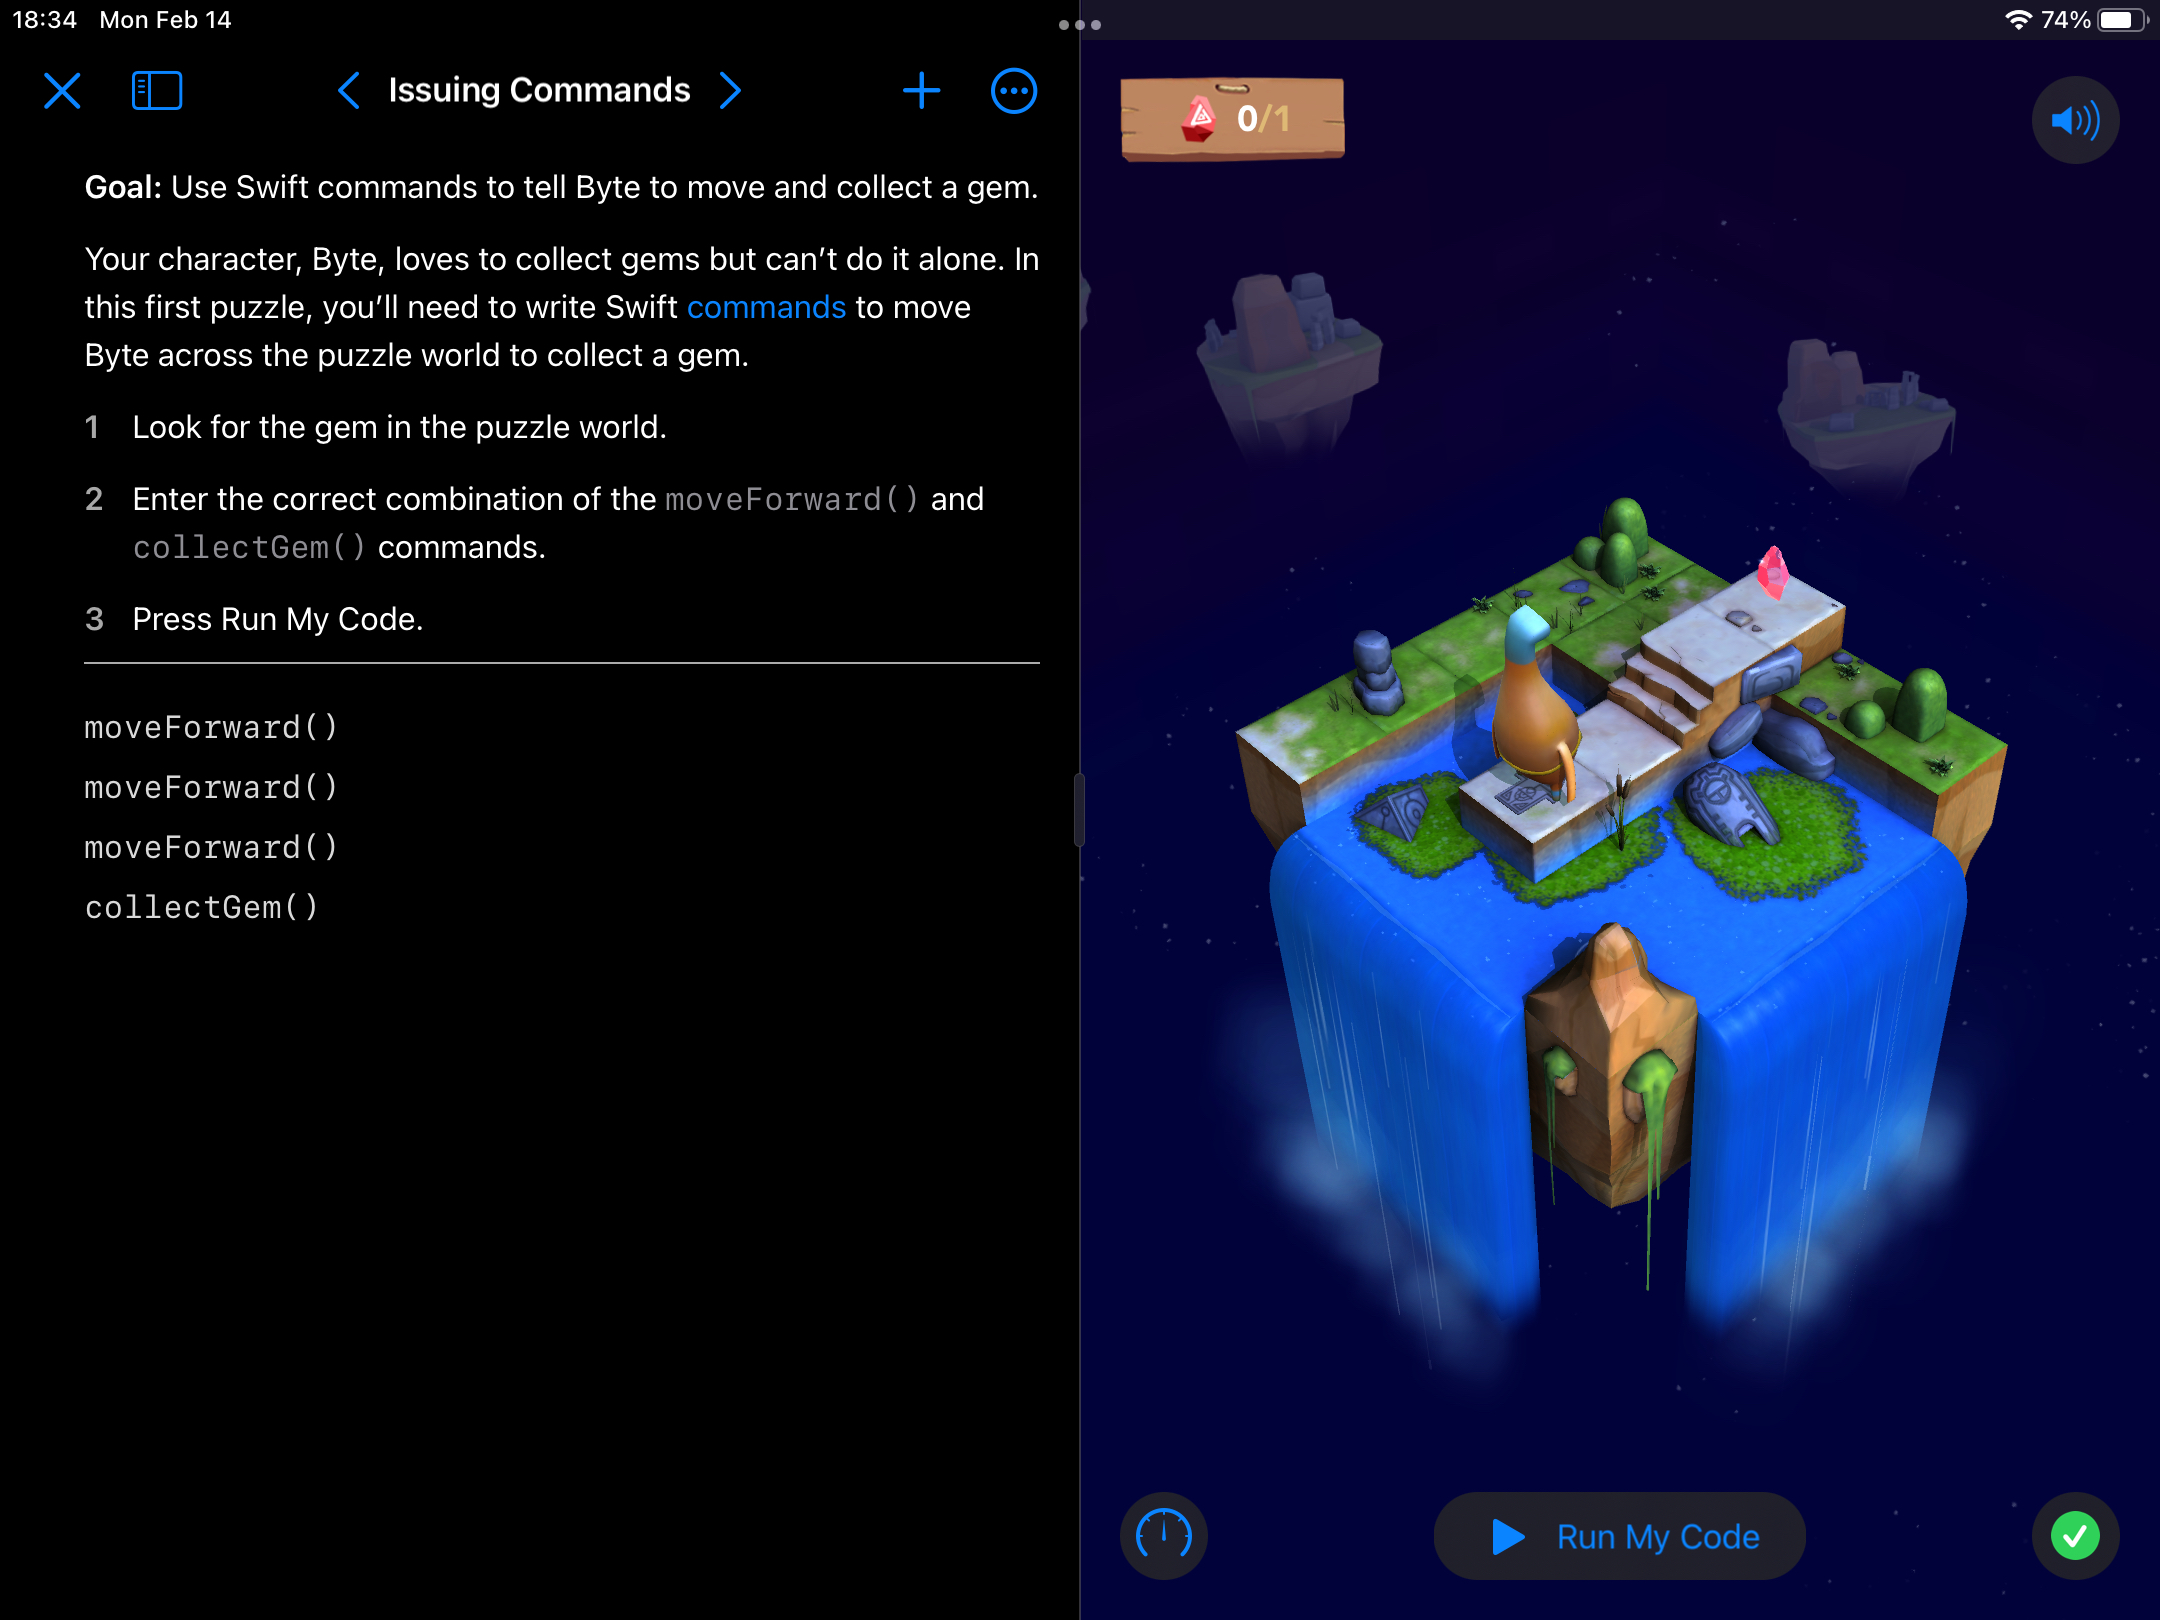
\includegraphics[width=1\textwidth]{images/Swift_Playground_iPad.jpeg}
\centering
\caption{\textit{Приказ апликације Swift Playgrounds на iPad-у}}
\label{slika:swift_playground_ipad}
\end{figure}

\begin{figure}[H]
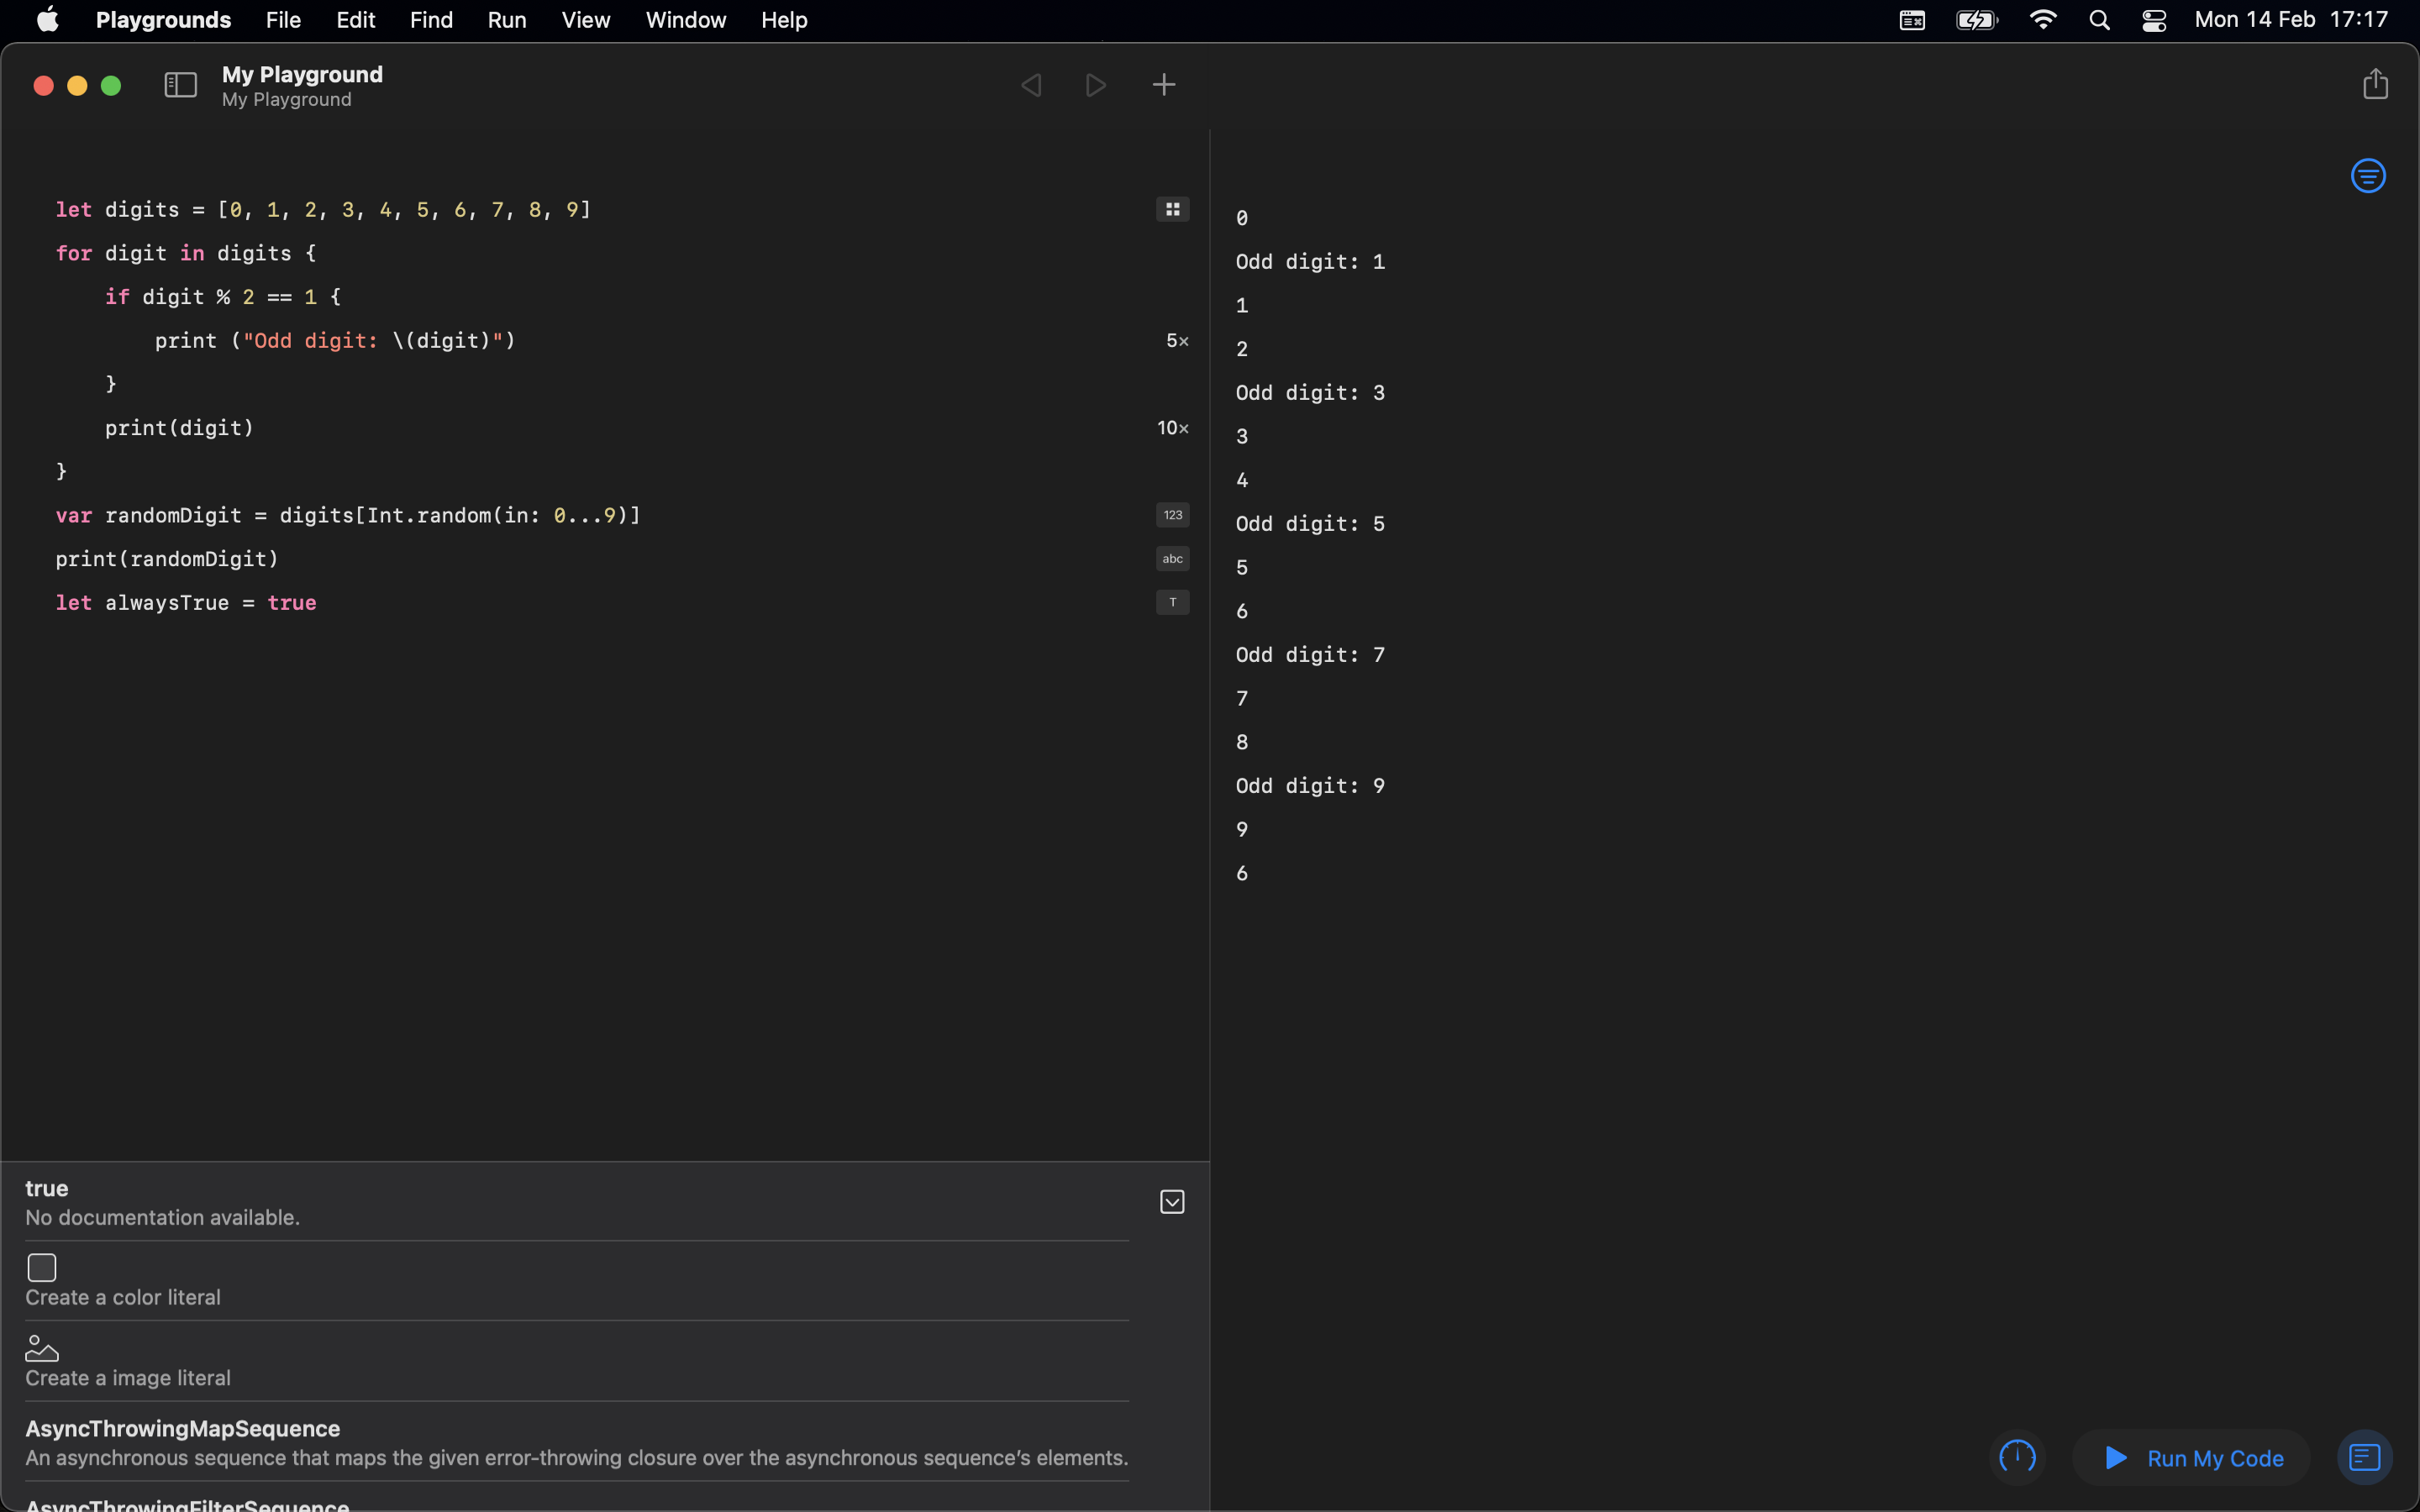
\includegraphics[width=1\textwidth]{images/Swift_Playground_macOS.png}
\centering
\caption{\textit{Приказ апликације Swift Playgrounds на macOS-у}}
\label{slika:swift_playground_macos}
\end{figure}

\subsection{\textit{Package manager}}

\textit{Swift package manager} је више-платформски алат за израду, покретање, тестирање и груписање ваших \textit{Swift} библиотека и извршних датотека. Помоћу менаџера пакета могу се најлакше поделити библиотеке и изворни кодови. Конфигурација самог менаџера као и сам \textit{Swift} менаџер података су такође писани у \textit{Swift}-у, чинећи конфигурацију циљаних извршних датотека и управљање зависностима међу пактима веома једноставним. 

\subsection{Компатибилан са \textit{Objective-C}-ом}

Цела апликација може бити написана у \textit{Swift}-у, или се \textit{Swift} може користити за додавање нових функционалности у већ постојећи програм. \textit{Swift} и \textit{Objective-C} могу узајамно постојати у апликацији, и корисник без проблема може користити делове кода написаног у једном језику унутар другог и обратно, уз само мало додатног подешавања пројекта које се може пронаћи на \textit{Apple}-вом сајту посвећеном развијаоцима софтвера (енг. developers) \cite{Apple_Developer}, конкретно на адресама \href{https://developer.apple.com/documentation/swift/imported_c_and_objective-c_apis/importing_objective-c_into_swift}{\textit{Importing Ojective-C into Swift}} и \href{https://developer.apple.com/documentation/swift/imported_c_and_objective-c_apis/importing_swift_into_objective-c}{\textit{Importing Swift into Objective-C}}.

\section{Xcode}
\label{sec:Xcode}

\indent \textit{Xcode} је интегрисано развојно окружење (ИРО) развијено од стране компаније \textit{Apple}, намењен оперативном систему \textit{macOS}. Софтвер је бесплатан и могуће је преузети га на \textit{Mac App Store}-у\footnote{Платформа која служи за дигиталну дистрибуцију апликација намењених оперативном систему \textit{macOS}}.

\subsection{Основно}

\indent ИРО \textit{Xcode} се користи за равој софтвера намењених оперативним системима \textit{iOS}, \textit{iPadOS}, \textit{watchOS}, \textit{tvOS} и \textit{macOS}. Прва верзија \textit{Xcode}-а, објављена је 2003. године, а последња стабилна верзија је \textit{Xcode}13. \textit{Xcode} укључује алат командне линије (енг. Command Line Tools, CLT) који омогућава \textit{UNIX} стил развоја софтвера помоћу терминала. На слици \ref{slika:xcode13_logo} може се видети званични лого ИРО-а \textit{Xcode}13.

\begin{figure}[H]

\includegraphics[width=1\textwidth]{images/Xcode_logo.jpg}
\centering
\caption{\textit{Званични лого ИРО-а Xcode13}}
\label{slika:xcode13_logo}
\end{figure}

\indent \textit{Xcode} се састоји од неколико алата који помажу програмеру приликом развоја апликација за \textit{Apple} платформе, од креирања апликације, преко тестирања и оптимизације, до прослеђивања на \textit{App Store}-у. Најзначанији алати који су део \textit{Xcode}-а су симулатор и инструменти.

\subsection{Симулатор}
\indent Симулатор се користи за тестирање апликације у току развоја уколико не постоји могућност употребе физичког уређаја. Тестирање на симулатору у неким ситуацијама може бити и боље јер пружа могућност тестирања апликације на више различитих уређаја (симулатора) одједном (на пример, различите генерације телефона \textit{iPhone}, као и различите верзије оперативног система). 
\\
\indent Као што је већ истакнуто, симулатор је део \textit{Xcode}-а; инсталира се уз њега, а покреће се и понаша као обична апликација оперативног система \textit{macOS} и омогућава симулацију свих уређаја са \textit{Apple} платформе (\textit{iPhone}, \textit{iPad}, \textit{Apple Watch}, \textit{Apple TV}). Приликом тестирања могуће је и покретање више симулатора за различите платформе да би се тестирала њихова компатибилност, као на пример сарадња апликације на \textit{iPhone}-у и \textit{Apple Watch}-у. 
Поред овога, још неке погодности које пружа симулатор су: интеракција са апликацијама коришћењем миша и тастатуре, одстрањивање неисправности у апликацији, оптимизација графичког приказа. На слици \ref{slika:simulatori} може се видети истовремена употреба симулатора телефона \textit{iPhone 13 Pro Max} са оперативним системом \textit{iOS} 15.0 и подешеном тамном бојом приказивања (енг. dark appearance), телефона \textit{iPhone SE - 2nd generation} такође са оперативним системом \textit{iOS} 15.0, али светлом бојом приказивања, таблета \textit{iPad Pro (9.7-inch)} са оперативним системом \textit{iOS} 12.0 и паметног сата \textit{Series 7 - 45mm} са оперативним системом \textit{watchOS} 8.0.

\begin{figure}[H]
\includegraphics[width=1\textwidth]{images/Simulators.png}
\centering
\caption{\textit{Приказ неколико симулатора}}
\label{slika:simulatori}
\end{figure}

\subsection{Инструменти}

\indent Инструменти су моћан алат, део \textit{Xcode}-a, који служе за анализу перформанси апликације као помоћ при њеном тестирању да би се боље разумело понашање апликације и омогућила додатна оптимизација перформанси. Коришћење инструмената од почетка развијања апликације доприноси раном откривању појединих грешака и олакшава њихово решавање. 
Неке од функција које инструменти омогућавају су:
\begin{itemize}
    \item Истраживање понашања апликације или процеса
    \item Испитивање карактеристика специфичних за уређаје као што су \textit{Bluetooth} и \textit{Wi-Fi}
    \item Профајлирање апликације у симулатору или на физичком уређају
    \item Анализа перформанси апликације
    \item Откривање проблема са меморијом
    
    \begin{itemize}
        \item Цурење меморије
        \item Напуштена меморија (енг. abandoned memory)
        \item Зомби објекти (деалоцирани објекти који се још увек чувају)
    \end{itemize}
    
    \item Оптимизовање апликације ради боље енергетске ефикасности
\end{itemize}

\section{SwiftUI}
\label{sec:SwiftUI}

\indent Део развоjа програмског jезика \textit{Swift} је усмерен ка поjедностављивању процеса израде корисничког интерфеjса и увођењу декларативне синтаксе у jезик. У том контексту настало jе радно окружење \textit{SwiftUI} коjе одликуjе могућност брзог креирања концизних и ефикасних решења.

\subsection{Уопштено}

\indent \textit{SwiftUI} је радно окружење које служи за израду апликација са графичким интерфејсом погодним за све \textit{Apple} платформе, користећи моћ програмског језика \textit{Swift} са што мање кода. Омогућава креирање разноврсних апликација уз само један скуп алата и програмског интерфејса апликације (енг. Application Programming Interface, API). 

\subsection{Основна структура}

\indent У склопу овог радног окружења добијамо велики број погледа (енг. views), контрола и распоредних структура (енг. layout structures) који олакшавају процес израде корисничког интерфејса апликације. Уз то садржи и алате за управљање током података од модела до погледа и контролера, које корисник види и може интераговати са њима преко додира, гестова и других типова улазних података у апликацији који се обрађују помоћу обрађивача догађаја. 
\\
\indent Структура апликације се дефинише помоћу протокола \textit{App} и попуњава се сценама које садрже погледе чији скуп чини кориснички интерфејс апликације. \textit{SwiftUI} омогућава и креирање нових погледа, једини услов је да тај поглед имплементира протокол \textit{View}. Нови поглед се може комбиновати са другим, корисничким или погледима радног окружења, као што су текстуална поља, слике и многи други да би се направили комплекснији погледи који ће бити погодни за све кориснике апликације.

\subsection{Карактеристике}

\indent Основна карактеристика која издваја радно окружење \textit{SwiftUI} од радног окружења \textit{UIKit} је другачија програмска парадигма, конкретно декларативна синтакса. Више о разликама ова два радна окружења биће описано у поглављу \ref{subsec:Разлика SwiftUI и UIKit} - \nameref{subsec:Разлика SwiftUI и UIKit}. 
\\
\indent Декларативна синтакса омогућава програмерима да што једноставније опишу понашање корисничког интерфејса. Код је много једноставнији за читање и разумевање као и за писање, чиме је обезбеђена значјна уштеда времена приликом писања новог кода и одржавања већ постојећег. Пример једноставног кода у \textit{SwiftUI}-у приказан је у делу \ref{lst:Пример SwiftUI кода} - \nameref{lst:Пример SwiftUI кода}. Модификатор \textit{@State} биће објашњен у делу \ref{subsec:Стање и ток података} - \nameref{subsec:Стање и ток података}.

\begin{lstlisting}[caption=\textit{{Пример SwiftUI кода}}, label={lst:Пример SwiftUI кода}, language=Swift, frame=single]
    // Ucitavanje SwiftUI radnog okruzenja
    import SwiftUI
    
    // Kreiranje strukture koja ce sadrzati glavni pogled
    struct Content : View {
    
        // Definisanje promenljive 'recepti'
        @State var recepti = RecepModel.listaRecepata
        
        // Definisanje tela pogleda
        var body: some View {
            // Izlistavanje svih recepata kroz tabelu
            List(recepti.stavke, action: recepti.izabranaStavka) { recept in
                // Prikaz slike
                Image(recept.slika)
                // Definisanje vertikalnog skupa elemenata
                VStack(alignment: .leading) {
                    // Prikaz teksta
                    Text(recept.ime)
                    // Prikaz teksta sive boje
                    Text(recept.vremePripreme)
                        .color(.gray)
                }
            }
        } 
    }
\end{lstlisting}

\subsection{Стање и ток података}
\label{subsec:Стање и ток података}

\indent Декларативно програмирање омогућаба да се за погледе вежу одговарајући модели података. Када год се неки од података промени, \textit{SwiftUI} аутоматски поново учита све погледе за који су промењени подаци везани и прикаже их кориснику, тако да програмер не мора да брине о томе. Ово се постиже променљивим стањима и везивањем, чиме се подаци везују за конкретне погледе. Тиме се остварује једини извор истине\footnote{Једини извор истине је начин структуирања информационих модела и шеме података тако да се сваки податак обрађује и мења на само једном месту} (енг. single source of truth, SSOT) за све податке и олакшава одржавање тачности података у сваком тренутку. 
\\
\indent У зависности од конкретне потребе у тренутној ситуацији, постоји више начина за остваривање јединог извора истине:

\begin{itemize}
    \item \textit{State} - Омогућава локално управљање стањем корисничког интерфејса, пример \ref{lst:Омотачи података - State} - \nameref{lst:Омотачи података - State}. Када је променљива означена као \textit{State}, другом погледу се мора проследити са префиксом '\$' уколико се жели омогућити промена њене вредности
    \item \textit{BindableObject} - Користећи \textit{ObservedObject} омотач својства, може се приступити спољашној референци на модел података који имплементира \textit{ObservableObject} протокол. Уколико је променљива смештена у спољашње окружење, може јој се приступити користећи \textit{EnvironmentObject} омотач својства. Инстанцирање посматрајућег (енг. observable) објекта директно у погледу, постиже се коришћењем \textit{StateObject}
    \item \textit{Binding} - Користи се за дељење референце на једини извор истине, пример \ref{lst:Омотачи података - Binding} - \nameref{lst:Омотачи података - Binding}
    \item \textit{Environment} - Подаци сачувани у \textit{Environment-у} се могу делити кроз целу апликацију, пример \ref{lst:Омотачи података - Environment} - \nameref{lst:Омотачи података - Environment}
    \item \textit{PreferenceKey} - Прослеђивање података уз хирархију погледа, од детета ка родитељу
    \item \textit{FetchRequest} - Управљање трајним подацима који се чувају унутар \textit{Core Data}
\end{itemize}

Графички приказ модификатора може се видети на слици \ref{slika:data_flow_primitives} - \nameref{slika:data_flow_primitives}.

\begin{figure}[H]
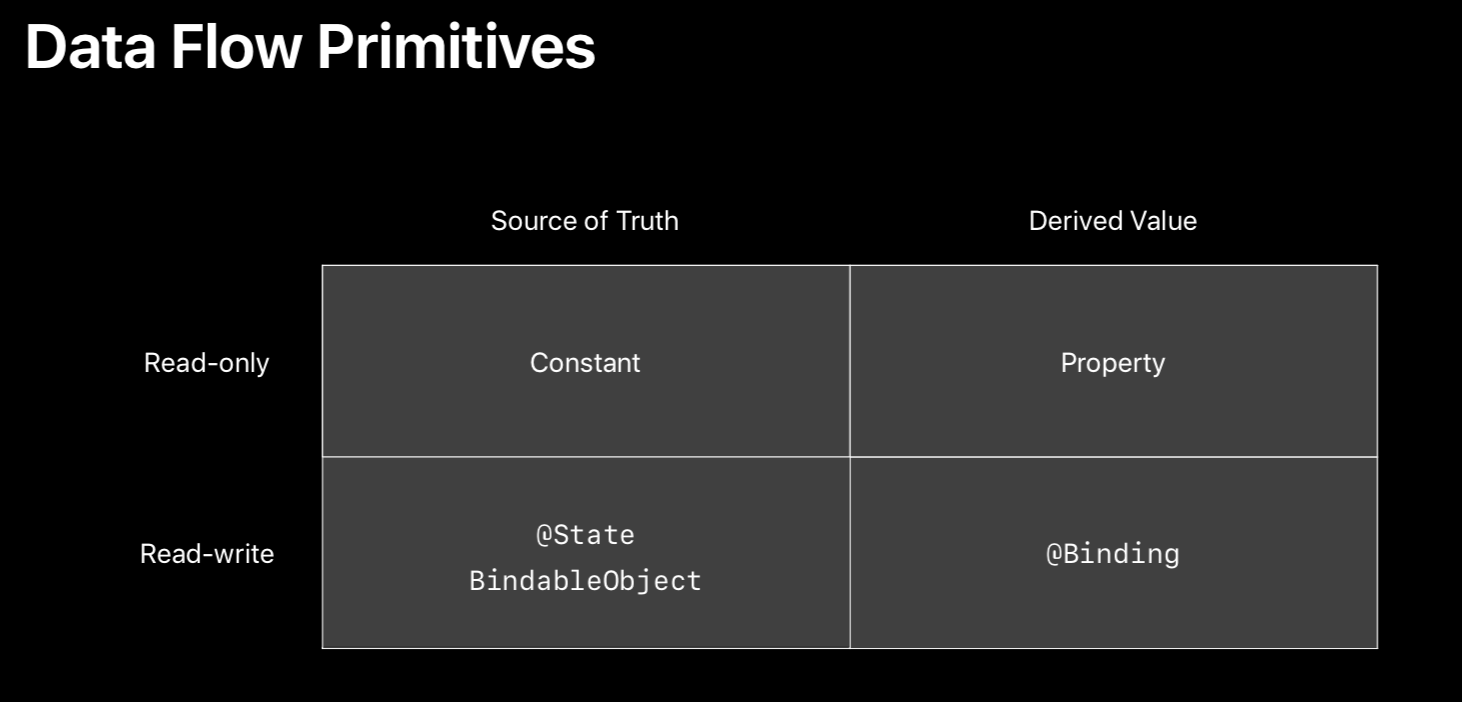
\includegraphics[width=1\textwidth]{images/DataFlowPrimitives.png}
\centering
\caption{\textit{Различити омотачи података}}
\label{slika:data_flow_primitives}
\end{figure}

\begin{lstlisting}[caption=\textit{{Омотачи података - State}}, label={lst:Омотачи података - State}, language=Swift, frame=single]
    struct Recept: View {
        var recept: ReceptPodatak
        @State private var daLiJeOmiljen: Bool = false
        
        var body: some View {
            VStack {
                Text(recept.ime)
                // 'OmiljenRecept' je pogled koji sadrzi zvezdicu koja oznacava da li je recept medju omiljenima (puna zvezdica - jeste, prazna - nije)
                OmiljenRecept(daLiJe: $daLiJeOmiljen)
            }
        }
    }
\end{lstlisting}

\begin{lstlisting}[caption=\textit{{Омотачи података - Binding}}, label={lst:Омотачи података - Binding}, language=Swift, frame=single]
    struct Recept: View {
    var recept: ReceptPodatak
    // Promenljiva 'daLiJeOmiljen' je definisana u jednom pogledu, a moze se menjati u drugom
    @Binding var daLiJeOmiljen: Bool

    var body: some View {
        Button(action: {
            // Akcija dugmeta koja menja promenljivu 'daLiJeOmiljen'
            self.daLiJeOmiljen.toggle()
        }) {
            // Provera promenljive 'daLiJeOmiljen' i prikaz odgovarajuce slike
            Image(systemName: daLiJeOmiljen ? "star.fill" : "star.empty")
        }
    }
}
\end{lstlisting}

\begin{lstlisting}[caption=\textit{{Омотачи података - Environment}}, label={lst:Омотачи података - Environment}, language=Swift, frame=single]
    struct Kulinarstvo_widgetEntryView : View {
    var entry: Provider.Entry
    
    // Cita podatke za 'widgetFamily' iz okruzenja aplikacije i smesta ih u promenljivu 'widgetFamily'
    @Environment(\.widgetFamily) var widgetFamily
    
    @ViewBuilder
    var body: some View {
        // U zavisnosti od promenljive 'widgetFamily' prikazuje se odgovarajuci widget
        switch widgetFamily {
        case .systemSmall:
            RecipeView(recipe: entry.recipe)
                .widgetURL(entry.recipe.url)
        case .systemMedium:
            RecipeMediumView(recipe: entry.recipe, ingredients: entry.recipe.ingredients.count > 3 ? Array(entry.recipe.ingredients.dropLast(entry.recipe.ingredients.count - 3)) : entry.recipe.ingredients)
        default:
            Text("")
        }
    }
}
\end{lstlisting}

\subsection{Разлика SwiftUI и UIKit}
\label{subsec:Разлика SwiftUI и UIKit}

\indent \textit{UIKit} и \textit{SwiftUI} су радна окружења развијена од стране \textit{Apple}-а, која помажу приликом израде корисничког интерфејса апликације. Генерално, највећа разлика између ова два радна окружења је у начину размишљања, како доћи до решења и како то решење касније имплементирати. Ова разлика ће најбоље бити показана на једном конкретном примеру: Форма за пријављивање на одређени сајт, креирање вертикалног скупа елемената, хоризонтално и вертикално центрираних у том скупу, скуп се састоји од два текстуална поља (корисничко име и лозинка) и једног дугмета (са акцијом провере података).
\\
\indent Са \textit{UIKit}-ом мора се водити рачуна о свим ситним детаљима као што су: креирање вертикалног скупа елемената, његово додавање у главни поглед, креирање текстуалног поља, додавање текстуалног поља у скуп елемената, додавање аутоматског ограничења распореда како би се центрирало текстуално поље, понављање поступка за друго текстуално поље и поновно понављање поступка за дугме. 
\\
\indent За разлику од \textit{UIKit}-а, \textit{SwiftUI} се базира на декларативном начину програмирања и коришћењем радног окружења \textit{SwiftUI} је довољно навести груписање два текстуална поља и дугмета у вертиклани скуп елемената и у ком погледу ће се приказати. Све ситне детаље ће радно окружење одрадити само, онако како је то уобичајено (енг. default) дефинисано. Наравно програмер по потреби може и сам променити ове детаље.
\\
\indent Креирање корисничког интерфејса у \textit{UIKit}-у коришћењем само \textit{Swift} кода је веома компликовано, и за веће пројекте готово немогуће. Најчешћи начин израде корисничког интерфејса је коришћењем \textit{Storyboards-а} i \textit{Interface Builder-а}, помоћу којих програмер креира кориснички интерфејс превлачењем, спустањем и конфигурацијом графичких елемената. У \textit{SwiftUI}-у се кориснички интерфејс изграђује помоћу \textit{Swift} кода. Једноставно се изјасни шта ће бити креирано и радно окружење то уради. Да би процес креирања био бржи и приступачнији, од верзије \textit{Xcode}-а 11, која је изашла у исто време када је представљен \textit{SwiftUI}, постоји могућност прегледа уживо сваког појединачног погледа који је креиран или скупа више погледа одједном. О овоме ће бити више речи у поглављу \ref{subsec:Xcode - преглед уживо} - \nameref{subsec:Xcode - преглед уживо}.
\\
\indent Уколико се сагледају архитектуре образаца, може се приметити да се \textit{UIKit} првенствено базира на \textit{MVC}\footnote{Архитектурни образац Модел-Поглед-Контролер (енг. Model-View-Controller) који се заснива на подели на три целине, модел - структура података, поглед - приказ података у корисничком окружењу, контролор - управљање моделом} обрасцу, док \textit{SwiftUI} користи \textit{MVVM}\footnote{Архитектурни образац Модел-Поглед-Модел погледа (енг. Model-View-ViewModel) који се заснива на подели на три целине, модел - структура података, поглед - приказ података у корисничком окружењу, модел погледа - стање података у моделу} образац. За заинтересоване читаоце, постоји могућност комбиновања ова два радна окружења и коришћење \textit{SwiftUI}-а унутар \textit{UIKit} кода, или обратно. Ова тема се оставља читаоцима да сами истраже како се то може постићи.

\subsection{Xcode - преглед уживо}
\label{subsec:Xcode - преглед уживо}

\indent Са представљањем \textit{SwiftUI}-a, \textit{Apple} је представио и нову верзију њиховог ИРО-а \textit{Xcode11}, у коме је додато својство рада у новом радном окружењу као и могућност прегледа уживо сваког погледа. Предност оваквог начина писања кода је пре свега у могућности брзог прегледа измена и то без поновног обнављања (енг. rebuilding) апликације, поготово уколико се ради на додавању или измени погледа који се налази дубоко унутар навигације апликације и за који је потребно више кликова и/или превлачења да би се до њега дошло. 
\\
\indent Преглед уживо помаже да се и у \textit{SwiftUI}-у користи метод превлачења и пуштања за креирање корисничког интерфејса, који се разликује од претходног који је коришћен унутар \textit{Storyboard}-а, јер сваки елемент се превлачи у део где се пише код и када се испусти тај елемент постаје део кода. Избор графичких елемената може се видети на слици \ref{slika:d&d1}, док је код програма и приказ уживо након испуштања графичког елемента \textit{Text} приказан на слици \ref{slika:d&d2}.

\begin{figure}[H]
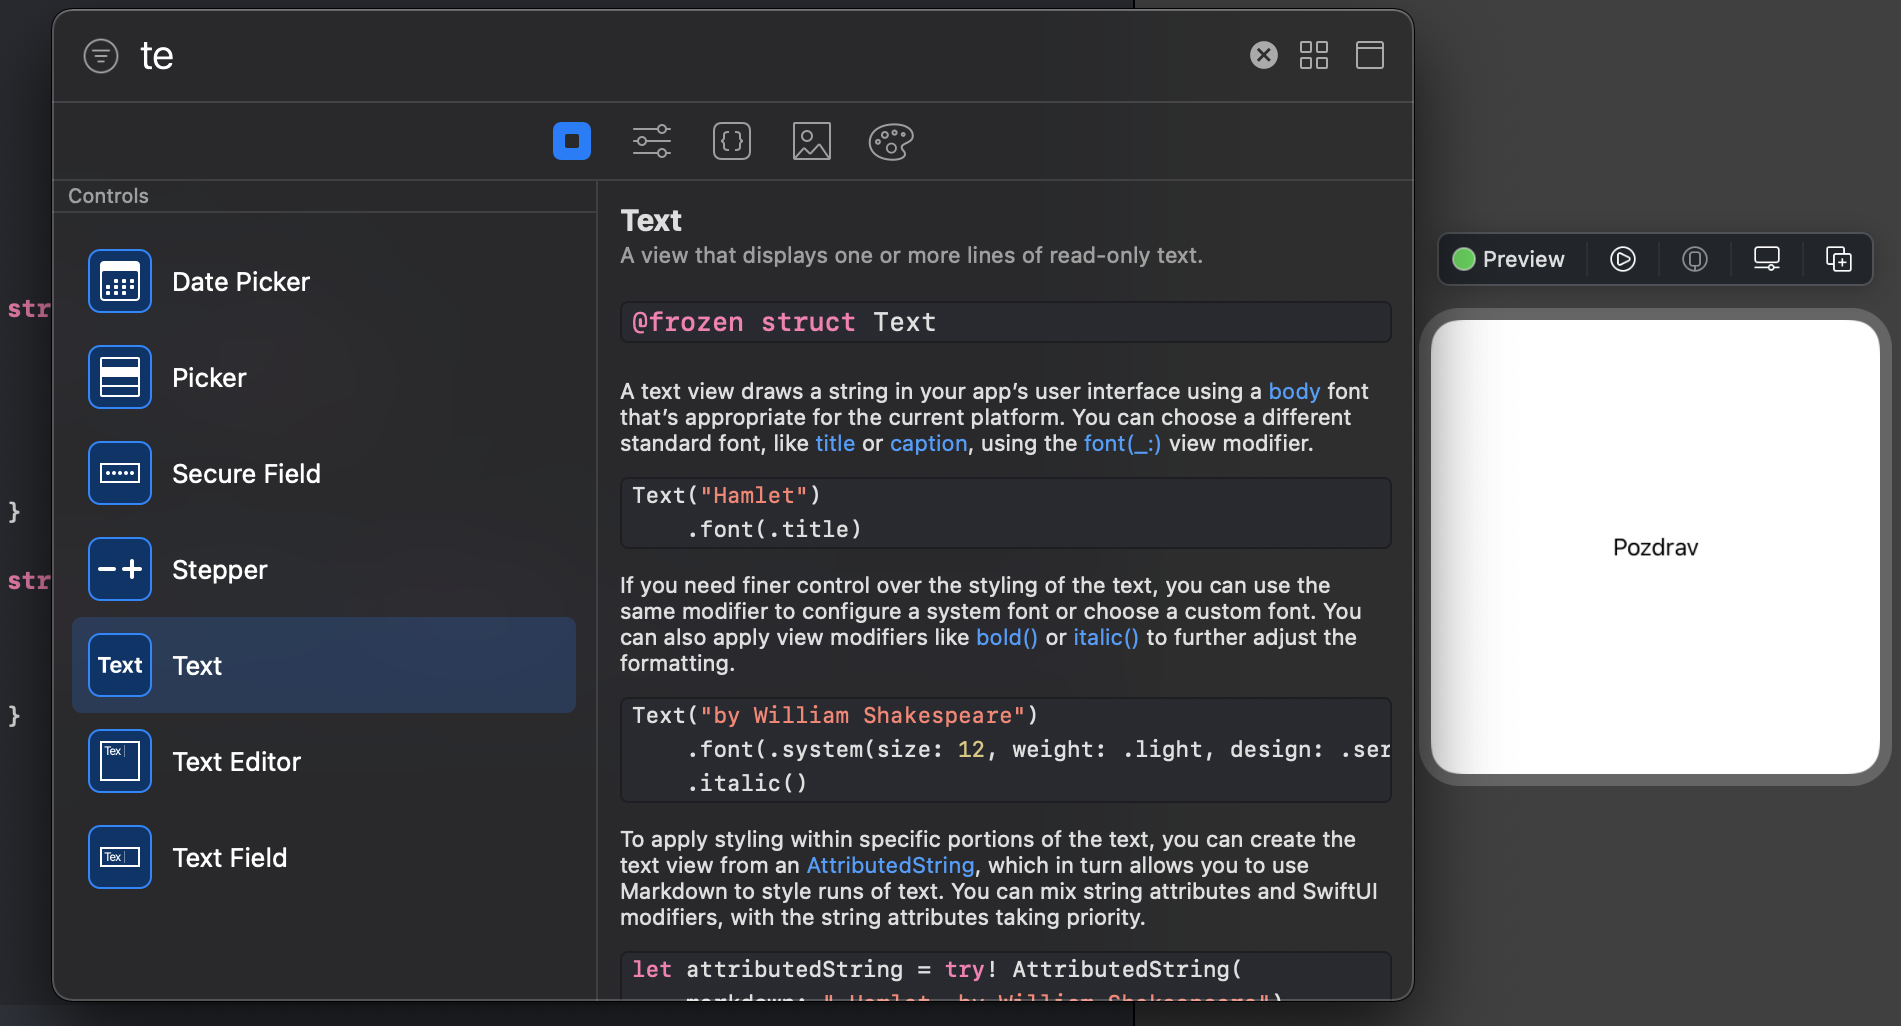
\includegraphics[width=1\textwidth]{images/Drag_and_drop_1.png}
\centering
\caption{\textit{Приказ графичких елемената}}
\label{slika:d&d1}
\end{figure}

\begin{figure}[H]
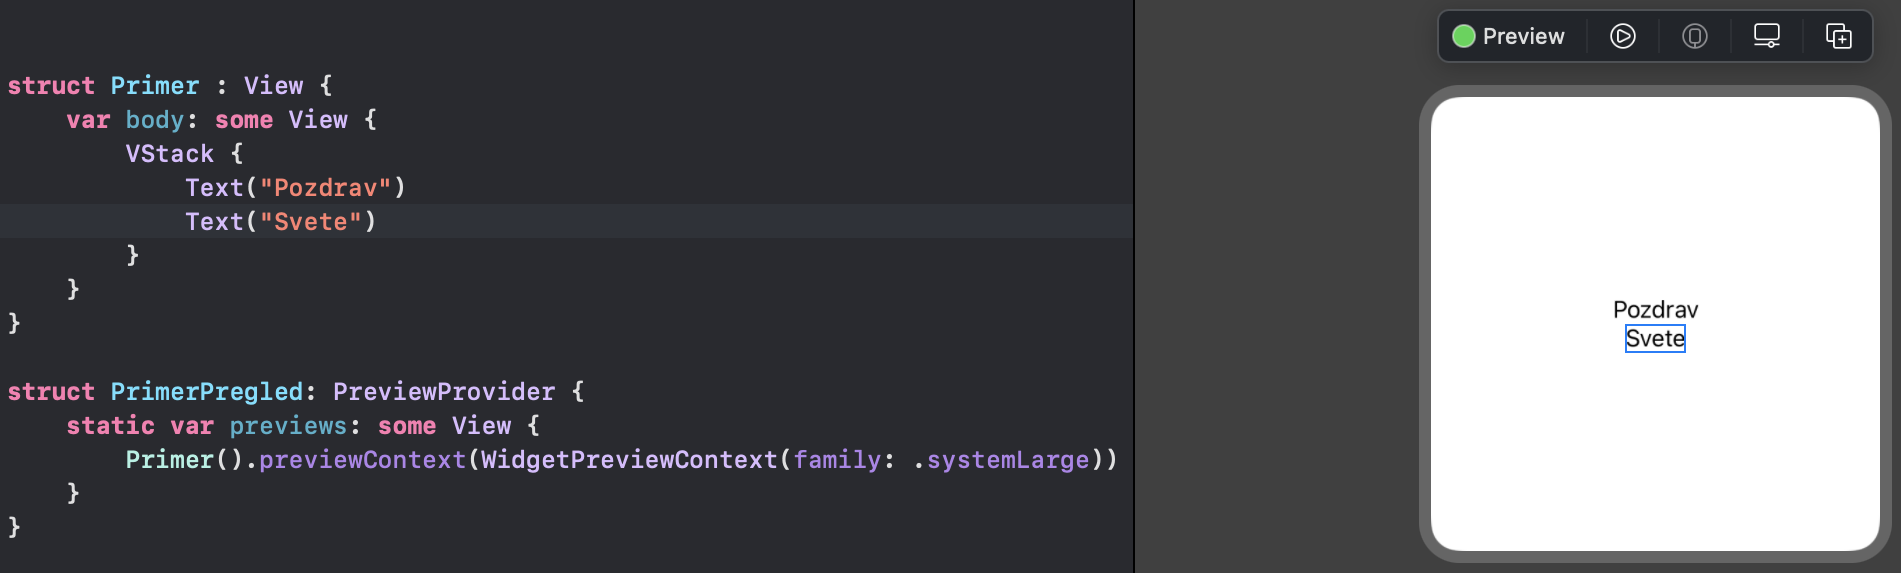
\includegraphics[width=1\textwidth]{images/Drag_and_drop_2.png}
\centering
\caption{\textit{Код програма након испуштања елемента}}
\label{slika:d&d2}
\end{figure}

Да би се омогућило коришћење приказа уживо, инстанца жељеног погледа се смешта унутар тела структуре која имплементира протокол \textit{PreviewProvider}, а која служи за живи приказ погледа или групе погледа. Пример употребе структуре која имплементира протокол \textit{PreviewProvider} може се видети у делу \ref{lst:Xcode - преглед уживо} - \nameref{lst:Xcode - преглед уживо}.

\begin{lstlisting}[caption=\textit{{Xcode - преглед уживо}}, label={lst:Xcode - преглед уживо}, language=Swift, frame=single]
    
    struct PlaceholderView : View {
        var body : some View {
            Kulinarstvo_widgetEntryView(entry: SimpleEntry(date: Date(), configuration: ConfigurationIntent(), recipe: RecipeModel.testData[0]))
        }
    }
    
    // Struktura u kojoj se konfigurise prikaz uzivo
    struct Kulinarstvo_widget_Previews: PreviewProvider {
        static var previews: some View {
            // Grupisanje vise pogleda
            Group {
                // Prikaz malog widget-a sa prvim elementom iz liste
                Kulinarstvo_widgetEntryView(entry: SimpleEntry(date: Date(), configuration: ConfigurationIntent(), recipe: RecipeModel.testData[0]))
                    .previewContext(WidgetPreviewContext(family: .systemSmall))
                
                // Prikaz srednjeg widget-a sa skrivenim sadrzajem
                PlaceholderView()
                    .previewContext(WidgetPreviewContext(family: .systemMedium))
                    .redacted(reason: .placeholder)
            }
        }
    }    
\end{lstlisting}

\indent Након сваке измене која се направи у коду који је везан за поглед(е) који се налази у прегледу уживо, \textit{Xcode} ће изнова направити нову верзију и покренути је у прозору за преглед уживо. Као што је виђено у примеру кода изнад, преглед уживо не мора приказивати само један поглед, већ се могу груписати различити погледи и сви бити приказати одједном. Предност оваквог приступа је могућност истовременог прегледа старог и новог изгледа погледа, више величина \textit{widget}-а, истих погледа са светлом и тамном бојом позадине, погледа на различитим језицима...

\indent За оне који желе да истраже више о овој теми, препорука је да одгледају два одлична клипа са \textit{Apple}-ове конференције за програмере из 2019. и 2020. године респективно. Клипови су: \href{https://developer.apple.com/videos/play/wwdc2019/233/}{\textit{'Mastering Xcode Previews'}} и \href{https://developer.apple.com/videos/play/wwdc2020/10149/}{\textit{'Structure your app for SwiftUI previews'}}.

\chapter{Улога и развој Widget-a}

\indent \textit{Widget}, као део мобилне апликациjе, се налази на почетном екрану уређаjа (телефона или таблета) и кориснику приказуjе одабране важне информациjе из те апликациjе. За разлику од \textit{widget}-а у оперативном систему \textit{Android}, коjи су присутни више од десет година, \textit{widgeti} на Apple платформама су уведени 2020. године, тако да jе и сама технологиjа коjа подржава њихово креирање и даље у активном развоjу.

\section{Основно}

\indent \textit{Widgeti} на уређајима са \textit{Apple} платформом узимају један од кључних делова апликације за коју је развијени и приказују га крајњим корисницима тамо где ће га најлакше уочити, на \textit{iPhone}-у и \textit{iPad}-у се може налазити на почетном екрану или у делу \textit{Today View}-а, док се на \textit{Mac} уређајима налазе у центру за нотификације. Величина \textit{widget}-а није флексибилна као на \textit{Android} уређајима, па тако постоји могућност креирања малих (величина 2x2 места на почетном екрану \textit{iPhone}-а), средњих (2x4) и великих (4x4), а од верзије оперативног система \textit{iPadOS15} екстра великих (4x8) (само за \textit{iPad} уређаје) \textit{widget}-а. 
\\
\indent Скуп свих тренутно доступних \textit{widget}-а на уређају налази се у галерији \textit{widget}-а (енг. widget gallery), која помаже корисницима приликом одабира конкретне величине и типа \textit{widget}-а (једна апликација може испоручити више типова \textit{widget}-а исте величине). Унутар галерије такође постоји опција за измену \textit{widget}-а у којој корисници могу да контролишу и мењају своје \textit{widget}-е и тиме их прилагоде себи, али само уколико је у току конструисања \textit{widget}-а од стране програмера то омогућено. Више речи о овоме биће у делу \ref{sec:Развој Widget-a} - \nameref{sec:Развој Widget-a}.
\\
\indent На оперативним системима \textit{iOS} и \textit{iPadOS} галерија има могућност додавања паметних гомила (енг. smart stack), које могу садржати до 10 различитих \textit{widget}-а исте величине. Паметна гомила у једном тренутку приказује један од \textit{widget}-а који се налазе у њој. Корисник може сам да мења који ће \textit{widget} бити приказан једноставним померањем (енг. scrolling). Временом, паметна гомила може научити који \textit{widget} корисник ставља на почетак гомиле у току дана (или недеље) и сама мењати примарне \textit{widget}-е у одређеном тренутку (на пример, након гашења аларма прво се приказује \textit{widget} са временском прогнозом, па најновије вести, стање у саобраћају...)
\\
\indent \textit{Siri} асистент\footnote{Интелигентни лични асистент на уређајима са \textit{Apple} платформом} може и сам додати \textit{widget}-е у паметну гомилу, уколико претпостави да постоји неки \textit{widget} који би кориснику био користан. Након тога, корисник сам одлучује да ли жели да новододати \textit{widget} остане у паметној гомили или не.

\subsection{WidgetKit}
\indent \textit{WidgetKit} је радно окружење које уз \textit{widget API} из  \textit{SwiftUI}-а служи за израду \textit{widget}-а, од његовог изгледа, преко временског ажурирања па све до омогућавања конфигурације \textit{widget}-а од стране крајњих корисника и управљања паметном гомилом приликом ротације \textit{widget}-а од стране система. Још једна могућност коју ово радно окружење пружа је повезивање апликације и самог \textit{widget}-а, што омогућава кориснику да отвори апликацију притиском на \textit{widget} и аутоматски оде на одговарајући поглед из \textit{widget}-а када жели да види детаљније податке. Мора се обратити пажња код оваквог начина комуникације јер \textit{widget} не би смео да служи само као пречица за покретање апликације, више о томе биће објашњено у делу \ref{sec:Дизајн Widget-a} - \nameref{sec:Дизајн Widget-a}.

\section{Развој Widget-a}
\label{sec:Развој Widget-a}
\indent \textit{Widget} је ништа друго до заправо само један \textit{SwiftUI} поглед. \textit{Widgeti} су тренутно једини део оперативних система \textit{Apple} платформи који у потпуности морају бити написани коришћењем радног оквира \textit{SwiftUI}. \textit{Apple} је отпочетка развоја \textit{widget}-а имао на уму овакву идеју, због начина приказивања података, само повременог ажурирања података и немогућности корисничке интеракције са самим \textit{widget}-има (осим једноставног клика којим се отвара одређени део аплиакције).

\subsection{Додавање widget додатка апликацији}
\indent Шаблон за \textit{widget} додатак креира основне компоненте потребне за његову израду. Унутар овог додатка корисник креира све потребне \textit{widget}-е за своју апликацију, независно од њиховог броја и величине. У специјалним ситуацијама различити типови \textit{widget}-а могу бити одвојени у посебним додатцима. Ово се најчешће односи када један тип \textit{widget}-а захтева одређене дозволе од стране корисника, док за други тип оне нису потребне (на пример, приступ тренутној локацији корисника).

\indent Кораци за креирање \textit{widget} додатка:
\begin{enumerate}
    \item Отворити пројекат у \textit{Xcode}-у и изабрати \textit{File -> New -> Target}
    
    \item Из групе \textit{Application Extension}, изабрати \textit{Widget Extension} и кликнути \textit{Next}
    
    \item Унети име додатка и изабрати тим који ради на пројекту
    
    \item Уколико \textit{widget} подржава конфигурацију од стране корисника, штиклирати поље \textit{Include Configuration Intent}
    
    \item Кликнути на \textit{Finish}
    
\end{enumerate}

\subsection{Додавање детаља конфигурације}
\indent Као што је већ напоменуто, шаблон \textit{widget} додатка пружа иницијалну имплементацију \textit{widget}-а која имплементира \textit{Widget} протокол. Два могућа начина конфигурације \textit{widget}-а су статичка (енг. StaticConfiguration) и конфигурација са сврхом (енг. IntentConfiguration). \\
\indent Статичка конфигурација се користи за \textit{widget}-е који немају параметре који могу бити конфигурисани од стране корисника (на пример, системска апликација \textit{Screen time} која води статистику о времену проведеном на одговарајућем уређају). Конфигурација са сврхом се користи за \textit{widget}-е чији одређени параметри могу бити конфигурисани од стране корисника (на пример, системаска аплиакција за временску прогнозу где корисник може наместити одређени град за који жели да добија податке). Ова конфигурација ће бити укључена и конфигурациони фајл ће бити додат уколико програмер приликом додавања \textit{widget} додатка штиклира поље \textit{Include Configuration Intent}.
\\
\indent Да би програмер спровео почетну конфигурацију \textit{widget}-а потребно је да проследи следеће параметре:
\begin{itemize}
    \item Тип (енг. Kind), стринг који идентификује \textit{widget}, требао би да казује шта \textit{widget} представља
    \item Снабдевач (енг. Provider), објекат класе која имплементира протокол \textit{TimelineProvider} и кроз временску линију коју производи одређује у ком тренутку ће \textit{widget} бити поново изрендерован и нови подаци бити приказани. Више о овом протоколу и свеукупној причи о временој линији у делу \ref{subsec:Временска линија} - \nameref{subsec:Временска линија}
    \item Затворење садржаја (енг. Content Closure), затворење које садржи \textit{SwiftUI} поглед и које \textit{WidgetKit} позива када дође време за поновно рендеровање садржаја \textit{widget-а}
    \item Прилагођена сврха (енг. Custom Intent), фајл који дефинише параметре које корисник може мењати и прилагођавати себи, више о овоме у делу: \ref{subsec:Intent} - \nameref{subsec:Intent}
\end{itemize}
Пример почетне статичке конфигурације \textit{widget}-а може се видети у коду \ref{lst:Widget - почетна конфигурација} - \nameref{lst:Widget - почетна конфигурација}. Да би се подесила боја шеме прослеђује се променљива '\textit{colorScheme}' којом се боја \textit{widget}-а усклађује са системском бојом уређаја. Променљива '\textit{kind}' служи за јединствену идентификацију типа \textit{widget}-а. 

\begin{lstlisting}[caption=\textit{{Widget - почетна конфигурација}}, label={lst:Widget - почетна конфигурација}, language=Swift, frame=single]
    struct KulinarstvoSecondWidget: Widget {
        @Environment(\.colorScheme) var colorScheme
        
        let kind: String = "KulinarstvoSlasnoIEfikasnoSecondWidget"
        
        var body: some WidgetConfiguration {
            StaticConfiguration(kind: kind, provider: SecondProvider()) { entry in
                KulinarstvoSecondWidgetEntryView(entry: entry)
            }
            .configurationDisplayName("Recept na klik")
            .description("Dodaj svoje omiljene recepte na pocetni ekran")
            .supportedFamilies([.systemLarge])
        }
    }
\end{lstlisting}

\subsection{Временска линија}
\label{subsec:Временска линија}
\indent Снабдевач временске линије генерише временску линију која се састоји од уноса (енг. entries), а сваки унос садржи датум и време када је потребно ажурирати садржај \textit{widget}-а. Када се датум и време из уноса подударе са реалним временом, \textit{WidgetKit} позива затворење садржаја које потом приказује ажуриране податке. 
\\
\indent Да би \textit{widget} био приказан у \textit{widget} галерији, \textit{WidgetKit} захтева од снабдевача преглед снимка (енг. Preview snapshot). Дохватање прегледа снимка се разрешава коришћењем променљиве '\textit{isPreview}' којом се проверава да ли снабдевач прегледа снимка шаље тренутни снимак за приказ у галерији или за приказ \textit{widget}-а на почетном екрану (или \textit{Today} у погледу, или у центру за обавештења). Када је параметар '\textit{isPreview}' тачан, \textit{widget} се приказује у галерији. Уколико за приказ \textit{widget}-а треба да буду приказани и одређени подаци, а подаци нису пристигли са серверске стране, постоје два решења. Могу се приказати подразумевани, унапред одређени подаци, или се могу користити подаци који чувају место правим подацима (енг. placeholder). У примеру \ref{lst:Widget - placeholder} - \nameref{lst:Widget - placeholder} може се видети креирање погледа чувара места (енг. placeholder view) коришћењем статичких података који су увек доступни, и конкретан приказ тог чувара места у прегледу уживо са сакривеним подацима (енг. redacted data) - приказ како ће корисник видети \textit{widget} док не пристигну конкретни подаци у неким ситуацијама.

\begin{lstlisting}[caption=\textit{{Widget - placeholder}}, label={lst:Widget - placeholder}, language=Swift, frame=single]
    struct PlaceholderView : View {
        var body : some View {
            Kulinarstvo_widgetEntryView(
                entry: SimpleEntry(date: Date(), configuration: ConfigurationIntent(), recipe: Datafeed.shared.favRecipes[0], parameterToShow: MainParameter.Sastojci.rawValue))
        }
    }
    
    struct Kulinarstvo_widget_Previews: PreviewProvider {
        static var previews: some View {
             PlaceholderView()
                .previewContext(WidgetPreviewContext(family: .systemLarge))
                .redacted(reason: .placeholder)
        }
    }
\end{lstlisting}

\indent Када пристигну подаци са сервера, снабдевач добија обавештење, сакупља реалне податке и приказује \textit{widget} са њима. Након што корисник дода \textit{widget} на почетни екран и буде приказан иницијални снимак изгледа \textit{widget-а}, \textit{WidgetKit} позива функцију \textit{getTimeline} из провајдера, чиме захтева временску линију.

\subsection{\textit{Intent}}
\label{subsec:Intent}
\indent \textit{Widget}-i предтављају погледе који не интерагују са корисницима, односно не подржавају интерактивне елементе, као што су поглед \textit{scroll} и дугме \textit{switch}. Једна врста интеракције корисника са \textit{widget}-ом постиже се омогућавањем конфигурације \textit{widget}-а од стране корисника коришћењем конфигурације \textit{Intent}, у којој се наводе сви параметри које корисник може да промени (и дозвољене вредности за те параметре). 
\\
\indent Да би се додали параметри које корисник може да конфигурише постоје предуслови који се морају испунити:
\begin{itemize}
    \item Додавање дефиниције \textit{intent}-а који дефинише конфигурабилне параметре 
    \item Коришћење протокола \textit{IntentTimelineProvider} уместо протокола \textit{TimelineProvider} као снабдевача временске линије, да би конфигурација параметара од стране корисника била сачувана у уносима временске линије
    \item Уколико параметри зависе од динамичких података потребно је имплементирати екстензију \textit{intent}-а
\end{itemize}
На слици \ref{slika:widget_configuration} се може видети како изгледа конфигурација \textit{widget}-а са два параметра, први за избор рецепта који ће у \textit{widget}-у бити приказан и избор примарног параметра уз опис рецепта (састојци или припрема).

\begin{figure}[H]

\includegraphics[width=0.5\textwidth]{images/Widget_configuration.png}
\centering
\caption{\textit{Конфигурација widget-а}}
\label{slika:widget_configuration}
\end{figure}

\subsection{Везе унутар \textit{widget}-а}
\indent Једини начин директне комуникације између корисника и \textit{widget}-а остварена је везама (енг. links) унутар \textit{widget}-а. Када корисник кликне на \textit{widget} отвара се апликација којој тај \textit{widget} припада, и може се конфигурисати који део апликације ће бити приказан кориснику у зависности од елемента унутар \textit{widget}-а на који је кликнуо. Свим величинама \textit{widget}-а може бити додат модификатор \textit{widgetURL(\_:)}, којим се одређује у који део апликације ће корисник бити одведен када кликне на \textit{widget}.
\\
\indent За све величине \textit{widget}-а, осим малих, може се користити и веза (енг. Link) која је додата једном погледу унутар \textit{widget}-а, којом је одређено место у апликацији које ће бити отворено (на пример, један \textit{widget} средње величине који садржи листу са 3 рецепата, сваки елемент листе има везу која води ка детаљној страни о рецепту који тај елемент представља). Иако \textit{widget} користи везе унутар својих елемената, може користити и модификатор \textit{widgetURL(\_:)}. Овај модификатор ће бити активиран уколико корисник кликне на поглед унутар \textit{widget}-а који нема дефинисану везу и биће отворена апликација без додатне навигације од стране \textit{widget}-а. У примеру кода \ref{lst:Везе унутар widget-а} - \nameref{lst:Везе унутар widget-а} приказана је употреба модификатора \textit{widgetURL(\_:)} за мале \textit{widget}-е, као и употреба веза за средње и велике \textit{widget}-е.

\begin{lstlisting}[caption=\textit{{Везе унутар widget-а}}, label={lst:Везе унутар widget-а}, language=Swift, frame=single]
    struct Kulinarstvo_widgetEntryView : View {
        var entry: Provider.Entry
        @Environment(\.widgetFamily) var widgetFamily
        
        @ViewBuilder
        var body: some View {
            switch widgetFamily {
            case .systemSmall:
                ImageRecipeView(recipe: entry.recipe, isSmallView: true)
                    .widgetURL(entry.recipe.url)
            case .systemMedium:
                Link(destination: entry.recipe.url ?? URL(fileURLWithPath: "")) {
                    RecipeMediumView(recipe: entry.recipe, listName: entry.parameterToShow)
                }
            case .systemLarge:
                Link(destination: entry.recipe.url ?? URL(fileURLWithPath: "")) {
                    RecipeLargeView(recipe: entry.recipe, mainParameter: entry.parameterToShow)
                }
            default:
                Text("")
            }
        }
    }
\end{lstlisting}

\subsection{Више \textit{widget}-а у једном проширењу}
\indent Уколико постоји потреба за коришћењем више различитих типова \textit{widget}-а у једном проширењу, то се може лако постићи уз само пар измена главног дела проширења, означеног анотацијом \textit{@main}. Уместо протокола \textit{Widget} главна структура мора имплементирати протокол \textit{WidgetBundle}. Тело структуре сада имплементира протокол \textit{Widget} и додата је анотација \textit{@WidgetBundleBuilder}. Приказ употребе више типова \textit{widget}-а у једном проширењу може се видети у примеру \ref{lst:Више widget-а у једном проширењу} - \nameref{lst:Више widget-а у једном проширењу}.

\begin{lstlisting}[caption=\textit{{Више widget-а у једном проширењу}}, label={lst:Више widget-а у једном проширењу}, language=Swift, frame=single]
    @main
    struct ReceptiWidgets: WidgetBundle {=
        @WidgetBundleBuilder
        var body: some Widget {
            DetaljanPrikazReceptaWidget()
            ListaRecepataWidget()
            SpisakZaKupovinuWidget()
        }
    }
\end{lstlisting}

\section{Дизајн \textit{Widget}-a}
\label{sec:Дизајн Widget-a}

\indent Главна улога \textit{widget}-а је приказивање садржаја који кориснику пружа корисне информације без покретања апликације. Самим тим подаци морају бити тачни и релевантни за корисника, сам \textit{widget} би требао бити конфигурабилан како би кориснику допустио одређену врсту слободе прилком коришћења и дизајниран тако да одговара апликацији којој припада.

\subsection{Фокус \textit{Widget}-a}
\indent  Подаци које \textit{widget} приказује треба да буду минималистички, да одговарају величини \textit{widget}-а (већа величина треба да повлачи и већу количину података) и да буду временски и кориснички релевантни. Први корак у дизајну \textit{widget}-а је избор дела аплиакције који ће тај \textit{widget} представљaти. 
\\
\indent Свака величина \textit{widget}-а која је омогућена за додавање из галерије треба да садржи одређену количину информација која је пропорционална тој величини. Не сме се дозволити да неколико величина \textit{widget}-а приказују исте податке, али истовремено приликом додавања нових података се мора водити рачуна о почетној идеји, односно делу апликације које тај \textit{widget} треба да представља. Уколико не постоји довољна количина података за веће \textit{widget}-е (на пример, за \textit{widget} величине \textit{large}), одређене величине могу бити искључене из понуде кориснику.
\\
\indent \textit{Widget} не би смео да служи само као пречица за покретање аплиакције. Корисници очекује од сваког \textit{widget}-а да им покаже корисне информације, у супротном неће наићи на добар одзив и истовремено може бити штетно самој апликацији (мањи број корисника, лошија оцена у продавници).

\subsection{Ажурни подаци}
\indent Да би \textit{widgeti} могли да пружају корисне и прецизне информације у скоро сваком тренутку, морају повремено бити ажурирани. \textit{Widgeti} не подржавају ажурирање у реалном времену, а и сам систем може ограничити ажурирање \textit{widget}-а у завиности од корисничког понашања и интеракције са њим, па се мора пронаћи начин на који ће подаци у \textit{widget}-у увек бити релевантни. 
\\
\indent Потребно је пронаћи оптимално време за ажурирање података у \textit{widget}-у, узимајући у обзир колико се сами подаци које \textit{widget} приказује често мењају. Једна корисна информација која се може приказати уз временски зависне податке је поље које ће представљати датум и време када су подаци последњи пут ажурирани. За одређене податке се може искористити помоћ система за одређивање датума и времена (на примеп, \textit{widget} који приказује време у које ће се огласити аларм, истовремено може приказивати и ажуран податак о томе колико је времена остало до оглашавања аларма).

\subsection{Конфигурабилност и интеракција}
\indent У већини случајева \textit{widget} треба да омогући кориснику конфигурабилност како би могао да пружио релевантне информације (на пример, књига коју корисник тренутно чита и његов прогрес у апликацији \textit{Apple Books}), док поједини \textit{widgeti} могу то изоставити (на пример, најновије вести). Уколико је \textit{widget} конфигурабилан, потребно је да подешавања буду једноставна и да се не захтева превише информација од корисника. Кориснички интерфејс за измену \textit{widget}-а је унапред одређен и исти за све \textit{widget}-е, као што је показано у делу \ref{subsec:Intent} - \nameref{subsec:Intent}.

\subsection{Дизајн прилагођен свима}
\indent \textit{Widgeti} треба да имају јарке боје како би се истицали на екрану, али истовремено и јасно видљив текст како би корисник могао да види све потребне информације након откључавања или непосредно пре закључавања уређаја. \textit{Widget} треба прилагодити апликацији коју представља (боје, фонт текста, јединствени елементи...), док истовремено не треба истицати превише елемената који ће указивати на аплиакцију (лого, име) јер се тиме само непотребно заузима простор унутар \textit{widget}-а који се може искористити на други начин.  
\\
\indent Количина информација коју ће бити приказана у \textit{widget}-у мора бити оптимална. Уколико се прикаже премало информација \textit{widget} неће имати превелики значај за кориснике, док превише информација на мало простора отежава читање и разумевање података.
\\
\indent Једна од битнијих ствари која се не сме заборавити у данашње време је дизајн \textit{widget}-а за обе врсте боја системске позадине (светле и тамне). Дизајн \textit{widget}-а се не сме разликовати од системске боје позадине јер ниједан корисник не жели видети таман текст на светлој боји позадине уколико је изабрао тамну системску боју позадине. Приликом израде обе врсте дизјна може помоћи \textit{Xcode preview} који омогућава истовремено сагледавање оба дизајна, упоређивање и исправљање евентуалних недостатака.
\\
\indent \textit{Apple} саветује да се никад не користи фонт текста мањи од 11 поена\footnote{\textit{Apple}-ов израз за "број који треба уписати у поље", универзална мера у дизајну на \textit{Apple} платформама}. Коришћење мањег фонта би корисницима знатно отежало употребу \textit{widget}-а. Поред овога, увек треба користити званичне елементе за приказ текста, како би се омогућила скалабилност као и системско читање текста. 
\\
\indent Пажњу треба обратити на дизајн прегледа \textit{widget}-а унутар галерије, за све типове и величине који \textit{widget} подржава, као и приказ чувара места уместо реалних података уколико они нису пристигли на време са сервера и непостоје подразумевани подаци. Уколико се исти елементи налазе у апликацији и истовремено на \textit{widget}-у потребно је да имају исту функционалност јер би у супротном корисници били збуњени. 
\\
\indent Потребно је искористити могућност приказа описа \textit{widget}-а у галерији и саставити кратак и јасан опис функционалности \textit{widget}-а. Груписање свих величина једног типа \textit{widget}-а са јединственим описом је погодно корисницима апликације, пре свега због једноставности разумевања коришћења \textit{widget}-а.
\\
\indent Скалабилност елемената унутар \textit{widget}-а је веома важна јер систем аутоматски прилагођава величину \textit{widget}-а величини екрана уређаја, зато је потребно обратити пажњу приликом додавања елемената. Најбоље је користити системске елементе који пружају флексибилност, у овом случају било који основни \textit{SwiftUI} елемент или њихова комбинација.

\chapter{Опис апликације}

\chapter{Закључак}

\literatura

\end{document}
